

% Colors
\definecolor{colorCellHighlight}{rgb}{0.85, 0.91, 0.97} % You can define Your own colors this way


% References
% Here You can choose the reference style

% ACM-style. Numeric references [1]. Alphabetical order.
% \usepackage[style=unitartucs/citations/numeric]{biblatex}

% IEEE-style. Numeric references [1]. Reference order.
\usepackage[style=unitartucs/citations/numeric,sorting=none]{biblatex}

% AMS-style. Trigraph references [ABC]. Alphabetical order.
% \usepackage[style=unitartucs/citations/alphabetic]{biblatex}

% APA-style. References with name and year (Koit 2010). Alphabetical order.
% \usepackage[style=unitartucs/citations/authoryear,uniquename=init]{biblatex}

\addbibresource{english/references.bib} % This file contains your bibliography entries


% Metadata
\title{State registry data access notifications for Estonian eID holders}
\author{Arkadi Statsenko}
\date{2025}
\supervisor{Daniel Würsch\degree{MSc}}% \and Co-Supervisor's name\degree{degree}}
\curriculum{Computer Science Curriculum}
\thesis{Bachelor's Thesis (9 ECTS)}
\keywords{Andmejälgija}


% Here begins the document

\begin{document}

\maketitle

\linespread{1.45} \selectfont

\newpage
\pdfbookmark[1]{\infoname}{info} % Adding the info page among the PDF bookmarks


% English information
\begin{info}
\begin{abstract}
\textit{Andmejälgija} is a protocol developed by Information System Authority (RIA), the purpose of which is to provide a uniform interface for querying Estonian residents' data access logs. There is also an \textit{Andmejälgija} web-view accessible from the state-portal \textit{\href{https://www.eesti.ee}{eesti.ee}}. 

The purpose of this thesis is to create a mobile application that would notify its users of updates in the access logs, letting them know that their data in some state database has been accessed. Implementation choices of different aspects of the solution are also going to be covered together with advantages and disadvantages of each. Additionally, the overview of the existing state databases will be provided, including whether they provide access logs or not.
\end{abstract}

% Visual abstract is not required for all curricula
%\begin{visualAbstract}
%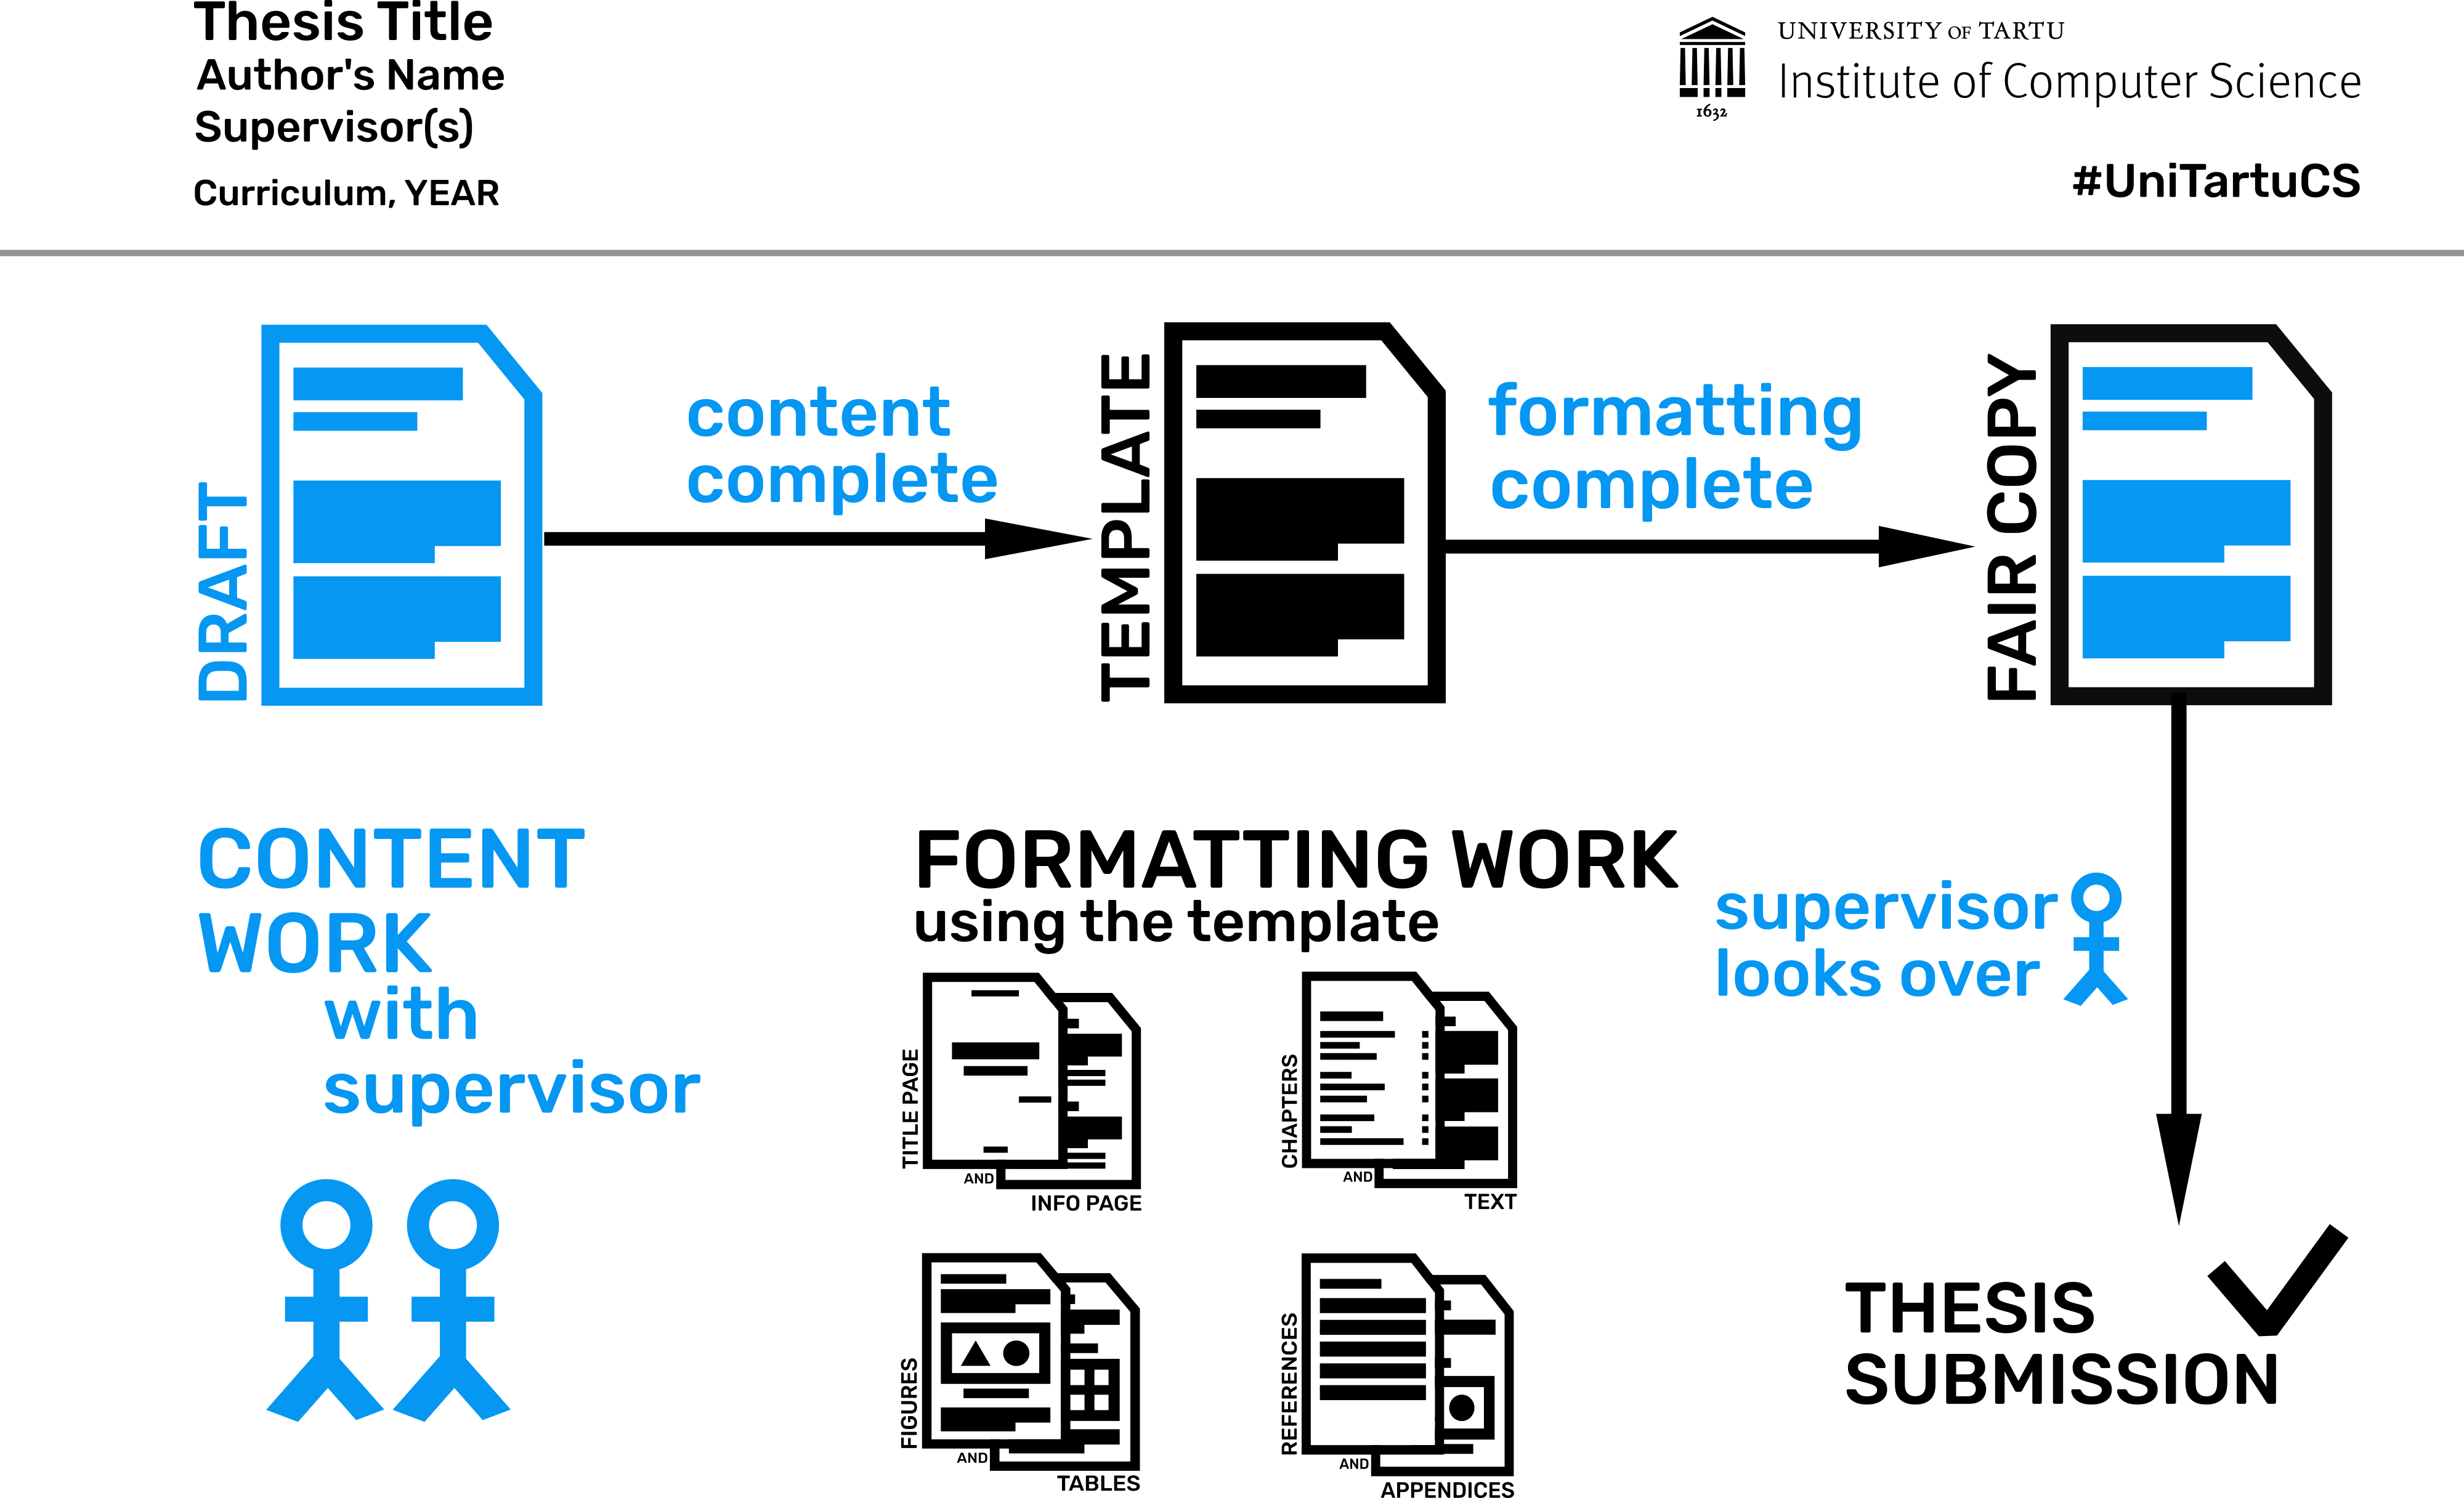
\includegraphics[width=\textwidth]{figures/Figure0-VisualAbstract.png}
%\end{visualAbstract}

% \keywords{}

\cercs{P170 Computer science, numerical analysis, systems, control  }
% Codes can be found at: https://www.etis.ee/Portal/Classifiers/Index/26
% Example: P170 Computer science, numerical analysis, systems, control
% Example: P175 Informatics, systems theory
\end{info}



% Estonian information
\begin{otherInfo}{estonian}{Teavitused riiklike andmekogude andmetele juurdepääsu kohta Eesti eID omanikele}
\begin{abstract}
Käesoleva lõputöö eesmärk on luua rakendus, mis teavitaks kasutajaid juurdepääsulogide uuendustest, andes neile teada, et nende andmeid mõnes riigi andmebaasis on kasutatud. Rakendusel on olnud erinevad rakendusvariandid, mida käsitletakse ka koos igaühe eeliste ja puudustega. Lisaks antakse ülevaade olemasolevatest riiklikest andmebaasidest, sealhulgas sellest, kas nad pakuvad juurdepääsulogisid või mitte.
\end{abstract}

% Visual abstract is not required for all curricula
%\begin{visualAbstract}
%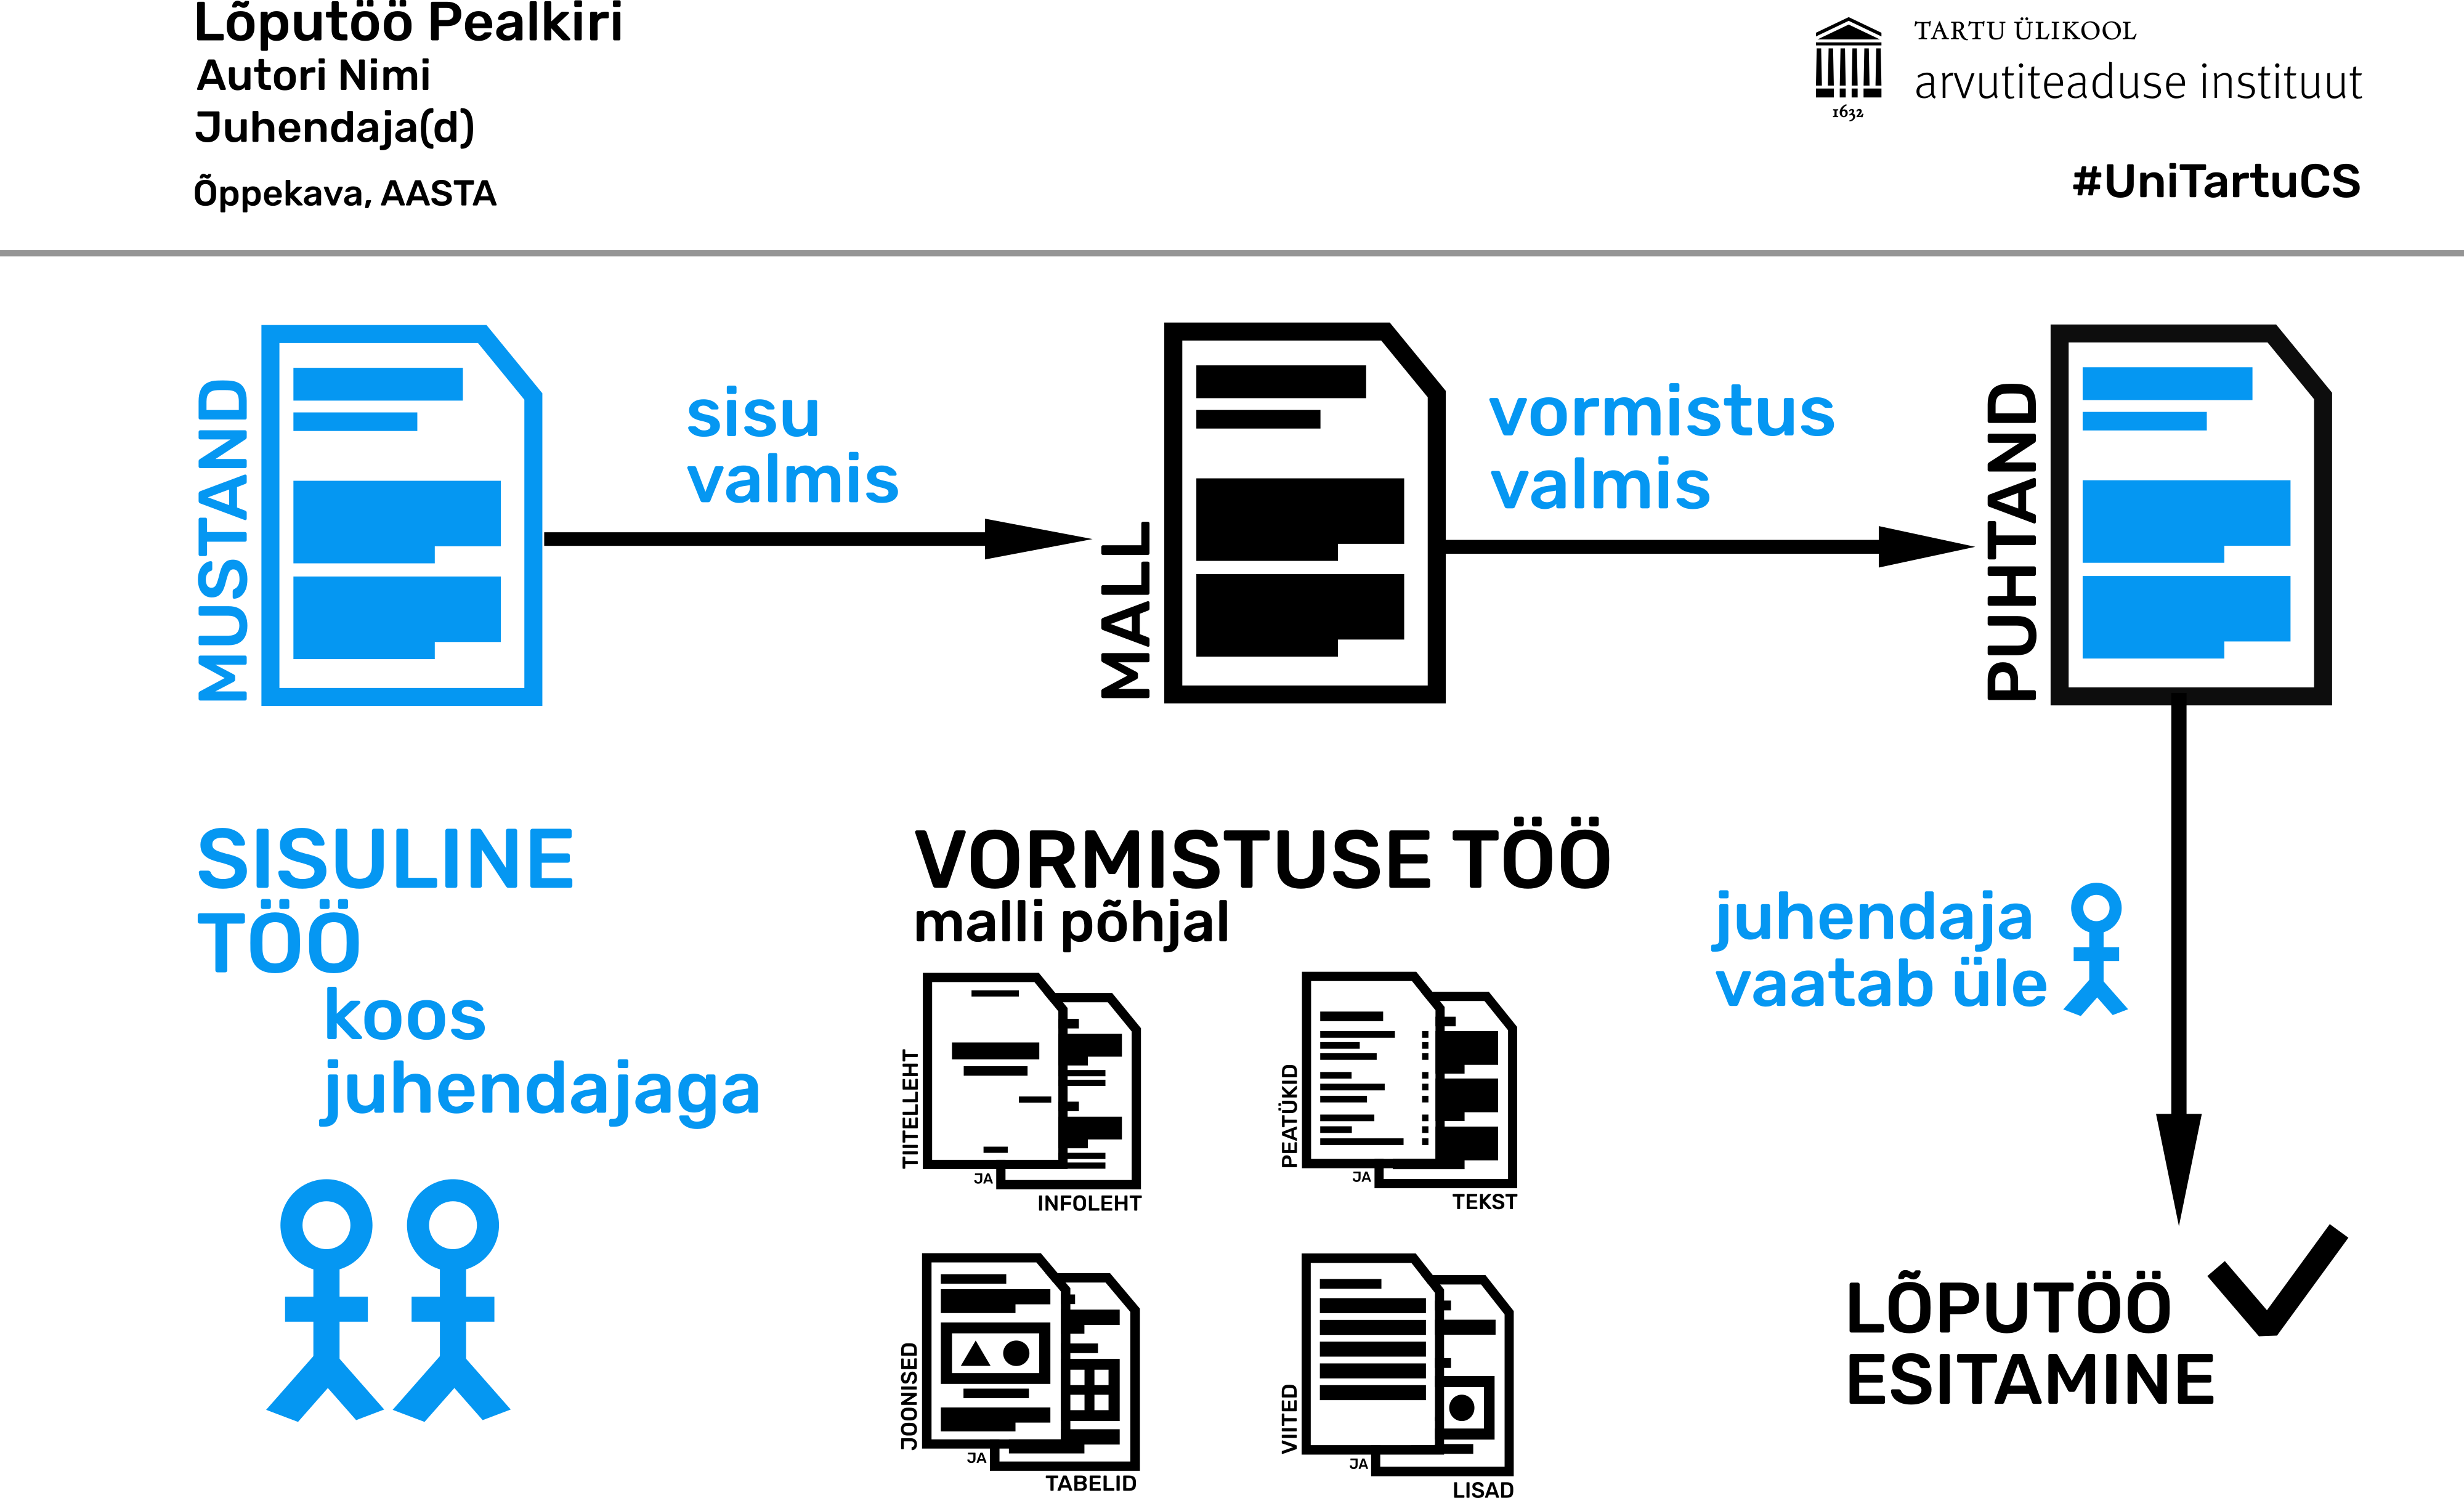
\includegraphics[width=\textwidth]{figures/Figure0-VisualAbstract-est.png}
%\end{visualAbstract}

% \keywords{}

\cercs{T170 Arvutiteadus, arvutusmeetodid, süsteemid, juhtimine (automaatjuhtimisteooria)}
\end{otherInfo}



\tableofcontents

\section{Introduction} \label{Introduction}

In Estonia there are a lot of state databases holding users' data, like Population Registry (\textit{Rahvastikuregister}) and Health Portal (\textit{Terviseportaal}). People's data in these databases is accessed by different parties for the variety of purposes. Usually those are legitimate purposes, like a doctor accessing person's health documents, or people themselves accessing their data in some information systems. However, sometimes the purpose of data access is not clear.

For the purposes of making the process more transparent, the Estonian Information System Authority (RIA) created a special service, Data Tracker (\textit{Andmejälgija}), in 2017, through which users can check which parties have accessed their data \cite{err-population-registry-unauthorized-access}. 

The Data Tracker is a people-oriented service on the state portal \textit{eesti.ee}, which aims to ensure transparency in the processing of personal data in both private and public sectors. The data tracker relies on the ability of each state database to store the data processing taking place within itself in the form of logs, in order to later display it to the individual, i.e. the data subject, via the service on \textit{eesti.ee} \cite{aj-github}.

Architecturally, it is a fully distributed system, i.e. the information displayed to the user comes directly from the database that implemented the Data Tracker service. At the user's request, \textit{eesti.ee} makes a query to each of the Data Tracker services and displays the query response without saving it \cite{aj-github}.

The Data Tracker should display to the individual information about data processing taking place locally in the database (activities of officials-employees or automated systems with personal data) as well as an overview of when data has been transferred to a third party (via X-Road to another government agency or private entity) \cite{aj-github}.

The Data Tracker doesn't notify, however, when the data is accessed by someone. In order to learn about the update in the data access logs, the person has to go to the \textit{eesti.ee} web-view and manually query access logs from specific databases. 

The primary objective of this thesis is to solve this problem by creating a mobile phone application that would notify its users about the new data access logs in near-real time. 

Additionally I would like to examine existing state databases processing people's personal data, including whether they provide access logs or not.
\section{Andmejälgija} \label{Andmejälgija}

\subsection{The protocol} \label{protocol_desc}

Andmejälgija is a protocol that state databases are responsible for implementing themselves. In order for the database to offer an \textit{Andmejälgija} service, they have to create an X-Road interface according to RIA specification\cite{aj-github-spec}. 

X-Road is a REST-based protocol which is used for secure data exchange between Estonian information systems over the Internet.

The \textit{Andmejälgija} X-Road interface is expected to have the following endpoints:

\textbf{\texttt{findUsage}}

A query searches the data recorder database for usage records that match the constraints given in the input. The output of the query returns all records found\cite{aj-github-spec}.

\textbf{\texttt{usagePeriod}}

The time period for which usage information can be requested\cite{aj-github-spec}.

\textbf{\texttt{heartbeat}}

Requesting the availability status of the tracker's usage information\cite{aj-github-spec}.

The overall architecture of the \textit{Andmejälgija} system is illustrated in Figure~\ref{fig:aj-model}, which shows how state databases interact with the \textit{eesti.ee} portal through X-Road to provide data access logs to end users.

\begin{figure}[H]
\centering
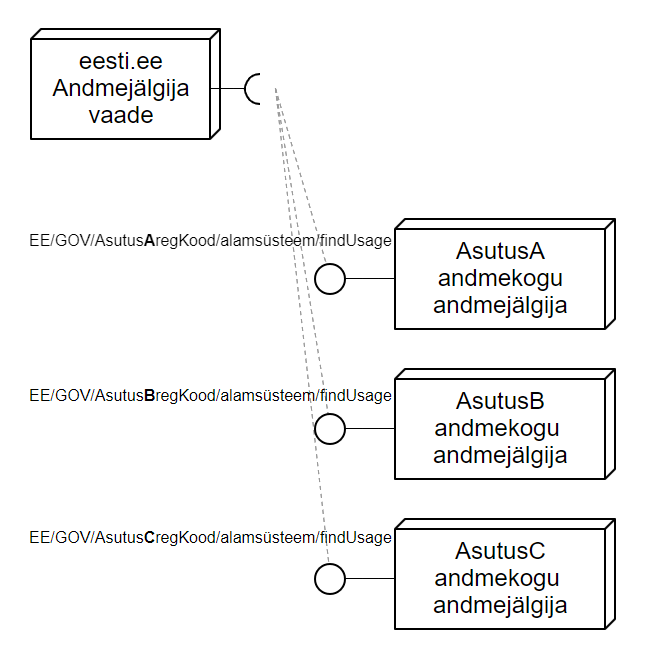
\includegraphics[width=450px]{english/figures/aj_model.PNG}
\caption{\textit{Andmejälgija} (Data Tracker) system architecture showing the interaction between entities implementing data tracking and \textit{eesti.ee} Data Tracker view. The data exchange happens via X-Road\cite{aj-github}.}
\label{fig:aj-model}
\end{figure}

\subsection{Usage}
There are several ways for end-users to access their Data Tracker data. State portal \textit{eesti.ee} provides a web-view for \textit{Andmejälgija} where end users can access their data access logs. Recently, RIA have also published a mobile application for \textit{eesti.ee}, that also features a view of data access logs. 

Another way to access Data tracker data is through Estonian Population Registry, although, is seems to be Population Registry specific as it doesn't provide access logs from other databases



\subsection{Adoption}
The current adoption of \textit{Andmejälgija} has some noticeable issues. Very often it is not at all clear why your data have been accessed, at least from the first glance. Explanation messages are vague and confusing, often being similar to "data access by personal code", making it difficult to understand the reason behind the data access, even if it was you who accessed it.

There is even an information sheet with recommendations for services implementing the \textit{Andmejälgija} protocol, and it states that providing poor quality explanations for data access is a bad practice.\footnote{\url{https://www.ria.ee/sites/default/files/documents/2022-11/Soovitusi-Andmejalgija-rakendamiseks.pdf}} 

\textbf{Good practice example:}

\begin{table}[H]
\centering
\begin{tabular}{|p{3cm}|p{6cm}|p{4cm}|}
\hline
\textbf{Data Processing Time} & \textbf{Activity} & \textbf{Party Receiving Personal Data} \\
\hline
13.01.2015 10:20:27 & Prescription viewed by doctor; prescription number 1018472350 & Doctor Viktor Pihlakas \\
\hline
19.01.2018 10:58:23 & Individual query for valid driver's licenses through state portal \textit{eesti.ee} & Jaan Kask 32405023456 \\
\hline
\end{tabular}
\caption{Example of good data access descriptions}
\end{table}

\textbf{Bad practice example:}

\begin{table}[H]
\centering
\begin{tabular}{|p{3cm}|p{6cm}|p{4cm}|}
\hline
\textbf{Data Processing Time} & \textbf{Activity} & \textbf{Party Receiving Personal Data} \\
\hline
13.01.2015 10:20:27 & PERSONAL DATA BY PERSONAL CODE & INSTITUTION X \\
\hline
19.01.2018 10:58:23 & INDIVIDUAL EXTENDED INFO QUERY BY PERSONAL CODE & FOUNDATION Y \\
\hline
\end{tabular}
\caption{Example of poor data access descriptions}
\end{table}

Apparently, the advice is often ignored, as many institutions tend to follow the bad example in practice. The thesis author's Data Tracker view is flooded with entries containing meaningless descriptions like the following:

\begin{table}[H]
\centering
\begin{tabular}{|p{2.5cm}|p{5cm}|p{3cm}|p{3.5cm}|}
\hline
\textbf{Date \& Time} & \textbf{Institution} & \textbf{Database} & \textbf{Activity} \\
\hline
02.08.2025 11:15 & Health and Welfare Information Systems Centre & Population Registry & INDIVIDUAL EXTENDED INFO QUERY BY PERSONAL CODE \\
\hline
01.08.2025 22:37 & Health and Welfare Information Systems Centre & Population Registry & INDIVIDUAL NAME RETRIEVAL BASED ON PERSONAL CODE \\
\hline
01.08.2025 20:23 & Education and Youth Board & Population Registry & PERSONAL DATA BY PERSONAL CODE \\
\hline
\end{tabular}
\caption{Extract from author's Data Tracker view demonstrating poor quality descriptions}
\end{table}

Furthermore, currently there is no law requiring institutions to implement the \textit{Andmejälgija} protocol, meaning that its use is pretty much voluntary.

In the following chapters I will cover different state databases and their implementations of \textit{Andmejälgija}, and whether they implement the protocol at all.
\section{Overview of state databases} \label{Overview of state databases}

\subsection{Databases implementing Andmejälgija}

\subsubsection{Digital Registry (Digiregistratuur)}
The Digital Registry demonstrates exemplary implementation of the Andmejälgija protocol. They provide very descriptive information about data access requests, making it clear to users why their data was accessed and by whom.

\subsubsection{Other databases implementing Andmejälgija}
\begin{itemize}
    \item Residence and Work Permit Register (Elamislubade ja töölubade register)
    \item Land Register (Kinnistusraamat)
    \item Professional Qualifications Register (Kutseregister)
    \item Taxpayers Register (Maksukohustuslaste register)
    \item Police Tactical Management Database (Politsei taktikalise juhtimise andmekogu)
    \item Agricultural Animals Register (Põllumajandusloomade register)
    \item Agricultural Subsidies and Land Blocks Register (Põllumajandustoetuste ja põllumassiivide register)
    \item Population Register (Rahvastikuregister)
    \item Prescription Centre (Retseptikeskus)
    \item Social Protection Information System (Sotsiaalkaitse infosusteem)
    \item Social Services and Benefits Register (Sotsiaalteenuste ja toetuste register)
    \item Labour Inspectorate Working Life Information System (Tööinspektsiooni tooelu infosusteem)
    \item Unemployment Insurance Database (Töötuskindlustuse andmekogu)
\end{itemize}

\subsection{Databases providing other form of data access tracking}

\subsubsection{E-File System (E-toimik)}
E-File System provides its own web-view for displaying requests made about the user, independent of the standard Andmejälgija protocol.
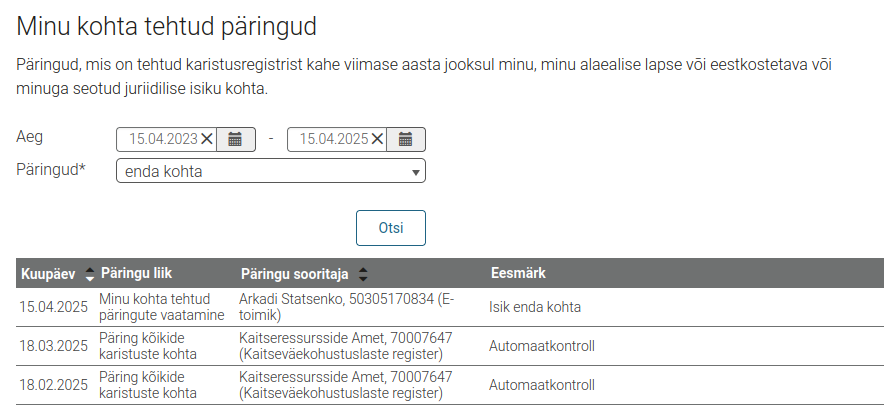
\includegraphics[width=450px]{english/figures/e-toimik.png}

\subsection{Databases not providing any kind of data access tracking}
\begin{itemize}
    \item Schengen Information System
    \item Border Control Database (Piirikontrolli andmekogu - PIKO)
    \item POLIS Information System (Infosusteem POLIS)
    \item Vehicle Registration Database (Liiklusregister)
    \item Court Information System (Kohtute infosüsteem - KIS)
    \item Employment register (Töötamise register (TÖR))

\end{itemize}



\section{Implementation}

\subsection{Description}

The main objective of this thesis has been to develop a solution that would notify users of data access events logged in the \textit{Andmejälgija} (Data Tracker) system. The resulting solution provides near real-time notifications when government institutions or other authorized entities access an eID holder's personal data.

\subsection{Discussion of implementation choice}
There are several possible approaches for developing such a solution. In this section different implementation options will be discussed, as well as their advantages and disadvantages.

\subsubsection{X-Road service}
\textit{Andmejälgija} specifications require entities responsible for the state databases to implement an X-Road interface themselves, as described in \ref{protocol_desc}, so one option would be to create an X-Road service that would query \textit{Andmejälgija} data over X-Road directly from those entities. The main advantage of this approach would be the freedom in how to notify users of changes to the access logs. As a server-based solution, the service could support various communication channels for delivering notifications to users, including instant messenger bots or e-mail notifications, for example. However, the list of requirements to operate such a service is daunting. 

\begin{itemize}
    \item {In order to join X-Road, a legal entity is needed.}
    \item {Permission has to be requested from every X-Road service you want to query data from. Specifically, considering that each information system is responsible for implementing the \textit{Andmejälgija} protocol themselves, the permission would be required from each entity responsible for the information systems from which the access logs would be requested.}
    \item {As part of X-Road network, one needs to operate a Security Server. For testing, it can be self-hosted on any hardware, but for production, a Hardware Security Module (HSM) is needed, in order to be compliant with eIDAS requirements. Obtaining or renting such hardware involves substantial financial investment. For example, a Thales Luna PCIe HSM A700 suitable for eIDAS qualified digital signing costs €8,990 (€10,877.90 incl. VAT) \cite{thales-luna-hsm-pricing}. Alternatively, renting a production ready Security server from Telia costs 210€ per month \cite{telia-xroad-server}}
    \item {Finally, considering that this approach would include creating a service that would store and transmit user's data, it would be required to follow strict regulatory requirements including the General Data Protection Regulation (GDPR). Staying compliant requires a continuous effort, and in case of failure to do so, there are harsh fines.}
\end{itemize}

Satisfying this criteria is difficult and expensive. Additionally, even with successful implementation, people would have to consent and entrust me with their data in order to be able to use the solution, which is not in the spirit of creating a solution for monitoring personal data access, as another data controller would be introduced.

\subsubsection{Standalone approach}
This approach uses the \textit{\href{https://www.eesti.ee}{eesti.ee}} session for accessing \textit{Andmejälgija} data. Once the user is logged in to the \textit{\href{https://www.eesti.ee}{eesti.ee}} state portal, certain internal API endpoints become available. Namely the \texttt{GET} endpoint \texttt{https://www.\href{https://www.eesti.ee}{eesti.ee}/\\andmejalgija/api/v1/usages} can be used to query \textit{Andmejälgija} data. The endpoint requires a parameter \texttt{dataSystemCodes} with which specific databases can be specified. For example, the GET request \texttt{/usages?dataSystemCodes=digiregistratuur\&\\dataSystemCodes=rahvastikuregister} would request access logs from \textit{Digiregistratuur} and \textit{Rahvastikuregister}.

The main advantage of this approach is the absence of all disadvantages of the X-Road approach: there are no legal requirements and the solution could be an open-source project, available for anybody to compile and use. There arises a problem, however. What about the notification part? Are users expected to set everything up on their hardware, including relevant communication channels? That would narrow down the project's user base to technical people knowing how to self-host, and having a server.

Consequently, creating a mobile application was determined to be the most optimal approach. A mobile application would keep the \textit{\href{https://www.eesti.ee}{eesti.ee}} session alive and poll the \textit{Andmejälgija} API. This approach combines ease of setup and use while keeping the solution standalone, without requiring a central server.

\subsection{Development}

First, the feasibility and reliability of the standalone approach had to be determined, especially as the approach would include a reverse-engineering of the user-facing service. The main challenge was to keep the session alive for as long as possible.

The \textit{\href{https://www.eesti.ee}{eesti.ee}} session is established using one of the strong authentication methods via the \textit{TARA} (Trusted Authentication and Authorization) service. Once the user is authenticated using ID-card, Mobile-ID, Smart-ID, or eID solution of another EU country, a JSON Web Token (JWT) token is issued, valid for 30 minutes. The session management is then handled by \textit{GovSSO} (Government Single Sign-On), which maintains the master server-side session token and imposes certain limitations as discussed in \ref{session-limitations}.

Once the user is authenticated, certain internal API endpoints become available, including those for refreshing the JWT token and getting \textit{Andmejälgija} access logs. The JWT refresh endpoint returns \texttt{Set-Cookie} headers that include an updated \texttt{JWTTOKEN} on success, with an updated expiration date (30 minutes from the moment of extension).

To test whether the session could be kept alive indefinitely, the Tab Reloader extension for Firefox by James Fray \cite{tab-reloader-addon} was used. Using this browser extension, the browser was configured to automatically reload the tab with the JWT token refresh endpoint. After the 8-hour experiment, the approach was deemed successful.

The next step was the development of the \textbf{Data Access Notifier} Android application. The reason why Android was chosen over iOS is that Android development is significantly more accessible for developers who do not own an Apple computer. Unlike iOS, Android development can be performed on nearly any modern computer with reasonably common operating system installed, including Linux.

The application was developed using the Kotlin programming language due to it being the new standard for developing Android applications \cite{kotlin-first}, as well as its more expressive syntax and promise of faster development speed.

The application is compatible with all Android versions starting from Android 8.1, meaning that it works on approximately 96.4\% of Android devices according to the Android Studio API version distribution chart shown in Figure~\ref{fig:android-api-distribution}.

\begin{figure}[H]
\centering
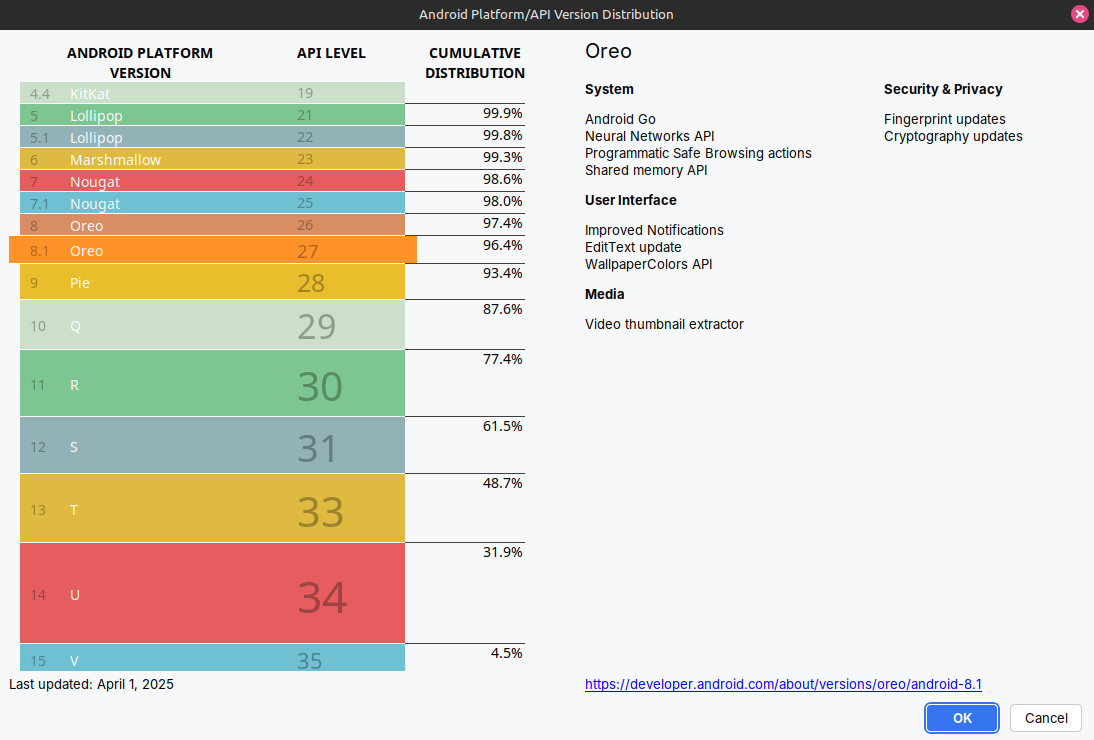
\includegraphics[width=450px]{english/figures/Screenshot from 2025-08-11 22-58-16.png}
\caption{Android Studio API Level Distribution for Android 8.1+ compatibility}
\label{fig:android-api-distribution}
\end{figure}

Currently, the application support is limited to Android 8.1 and higher. While support for iOS and other platforms is not planned due to limited development time and resources, anybody who deems this solution useful is encouraged to port it to platforms other than Android.

\subsubsection{Licensing}
The \textbf{Data Access Notifier} application is released as open-source software under the MIT License. This simple and permissive license allows users to freely use, modify, and distribute the software for both commercial and non-commercial purposes. 

The choice of MIT License aligns with the project's goal of providing a transparent and accessible solution for personal data monitoring, enabling the broader community to contribute to and benefit from the development efforts without strict licensing barriers.

\subsubsection{Authentication}
To gain access to \textit{\href{https://www.eesti.ee}{eesti.ee}} internal APIs, the user needs to be authenticated via the State Authentication Service (\textit{TARA}). The initial plan was to reverse engineer the authentication flow and authenticate the user by sending raw HTTP requests and handling responses. This approach, however, would be fragile and require substantial engineering effort to develop and maintain due to the flow being fairly complex and prone to unannounced changes to \textit{TARA}.

Instead, it was decided to use Android WebView for authentication as a more reliable and convenient approach for both the user and the developer. By leveraging WebView, the \textbf{Data Access Notifier} application can present the official \textit{TARA} login page directly to the user, allowing them to authenticate using their preferred method (ID-card, Mobile-ID, Smart-ID, or eID of another EU country). This approach significantly reduces the risk of breaking changes due to updates on the \textit{\href{https://www.eesti.ee}{eesti.ee}} or \textit{TARA} platforms. Once the user is authenticated, the application can access the necessary session cookies and JWT token to interact with the internal APIs.

\subsubsection{Interacting with \textit{\href{https://www.eesti.ee}{eesti.ee}} internal APIs}
For interacting with \textit{\href{https://www.eesti.ee}{eesti.ee}} internal APIs, the OkHttp library by Square, Inc.\cite{okhttp-library} was used. The following API endpoints were utilized:

\begin{itemize}
    \item \textbf{GET} \texttt{https://www.\href{https://www.eesti.ee}{eesti.ee}/timur/jwt/extend-jwt-session}
    
    An endpoint for extending JWT session.
    
    \item \textbf{GET} \texttt{https://www.\href{https://www.eesti.ee}{eesti.ee}/andmejalgija/api/v1/usages}
    
    An endpoint for querying Data Tracker access logs.
    
    Query parameters:
    \begin{itemize}
        \item \texttt{dataSystemCodes}: The name of the information system the access logs are queried from.
    \end{itemize}
    
    \samepage
    Response body format (JSON):
    \begin{listing}[H]
    \begin{minted}{json}
{
  "findUsageResponses": [
    {
      "logTime": "2025-08-03T22:40:47",
      "receiver": "Tervise ja Heaolu Infosüsteemide Keskus",
      "infoSystemCode": "rahvastikuregister",
      "action": "ISIKU NIME VÄLJASTAMINE ISIKUKOODI PÕHJAL"
    },
    // more objects to follow
  ]
}
    \end{minted}
    \caption{API response format for Andmejälgija usage data}
    \label{lst:andmejalgija-response}
    \end{listing}
    
    Response fields:
    \begin{itemize}
        \item \texttt{logTime}: Timestamp of the data access event in ISO 8601 format
        \item \texttt{receiver}: Entity that accessed the data
        \item \texttt{infoSystemCode}: The information system where the data has been accessed.
        \item \texttt{action}: Description of the action performed (in Estonian)
    \end{itemize}
\end{itemize}

Both endpoints require a valid JWT token to succeed. WebView's \texttt{CookieManager} serves as a single source of truth in this application, where all cookies are loaded from for making requests and written to upon receiving responses.

\subsubsection{Keeping the session alive}
The API requests are authenticated using a JWT token cookie, the lifetime of which is 30 minutes. This means that the \textbf{Data Access Notifier} application must either run a continuous foreground service or be awakened periodically to request an updated JWT token and send requests to \textit{Andmejälgija}.

On Android, there are several ways to accomplish this, although it is worth mentioning that Android is very restrictive regarding background tasks and battery usage. Several approaches were tried and the experience with them in the context of developing this application will be described.

\subsubsection{WorkManager approach}
According to the Android documentation, WorkManager is the recommended solution for persistent work \cite{android-persistent-work}. Work is persistent when it remains scheduled through application restarts and system reboots. This seemed to describe the use case very well, so this was the first approach that was tried.

Work is defined in WorkManager using a WorkRequest. There are several WorkRequest types available, including \texttt{PeriodicWorkRequest} and \texttt{OneTimeWorkRequest}.

Using \texttt{PeriodicWorkRequest}, it is possible to schedule periodic tasks. The important limitation here is that it is not possible to schedule a task to execute more frequently than every 15 minutes. While this may sound appropriate for the use case of having to renew the session at least every 30 minutes, in practice, the situation is different.

During development, a critical difference between session handling in web browsers versus HTTP client libraries was discovered. While the browser-based testing with Tab Reloader successfully maintained the session by refreshing the JWT token every 15 minutes, the same approach using OkHttp in the Android application failed to keep the session alive.

The exact cause of this discrepancy remains unclear. It appears that the \textit{\href{https://www.eesti.ee}{eesti.ee}} session management system expects more frequent interaction or handles cookie management differently when requests originate from HTTP client libraries compared to full web browsers. Indeed, with shorter intervals of 5 minutes, the session remains alive. This behavioral difference rendered the \texttt{PeriodicWorkRequest} approach with 15-minute intervals unsuitable for maintaining persistent sessions in the application context.

While \texttt{OneTimeWorkRequest} is designed for one-time tasks, it is possible to chain them by having each one-time work create another one-time work at the end of its lifespan. This approach allows setting custom intervals shorter than 15 minutes, circumventing the limitation imposed by \texttt{PeriodicWorkRequest}.

While \texttt{OneTimeWorkRequest} may appear to be a suitable solution, WorkManager itself proved to be rather unreliable for the use case after testing. The limitation of WorkManager is that tasks scheduled by it are managed by the system and may be deferred if deemed necessary by the Android system. For example, tasks may not execute if the phone has low battery level, or even in other scenarios depending on the aggressiveness of the Android variant regarding the restrictions imposed on application behavior.

\subsubsection{Foreground service approach}
A foreground service is one of the most reliable types of tasks an application can schedule. In contrast to background services, foreground services are considered to be of higher priority by the system and thus are not candidates for termination when the system is low on memory or the phone has low battery level.

However, an important limitation has been introduced in recent Android versions. More specifically, starting from Android 15, the system places restrictions on how long certain foreground services are allowed to run while the application is in the background. Currently, this restriction only applies to \texttt{dataSync} and \texttt{mediaProcessing} foreground service types. The foreground services of those types are allowed to run for a total of 6 hours in a 24-hour period \cite{android-15-datasync-timeout}.

The most appropriate foreground service type for the use case is \texttt{dataSync}, meaning that it falls under the 6-hour per day restriction. While it should be possible to choose an arbitrary foreground service type regardless of the actual task type, doing so is not the cleanest approach, especially considering the existence of better alternatives. Furthermore, doing so may also impact the application's acceptance into the Google Play Store.

\subsubsection{Hybrid AlarmManager approach}
\label{alarmmanager-approach}
After evaluating the limitations of WorkManager and the restrictions on foreground services, a hybrid approach combining AlarmManager with a \texttt{dataSync} foreground service was ultimately adopted. AlarmManager is a system service that allows scheduling operations to be executed at specific times, even if the application is not running. By using AlarmManager to trigger the application at regular intervals (e.g., every 5 minutes), it is ensured that the session renewal and data polling tasks are reliably executed.

When the alarm fires, the application starts a short-lived \texttt{dataSync} foreground service to perform the necessary network operations: refreshing the JWT token and querying the \textit{Andmejälgija} API. This approach leverages the reliability of foreground services for critical tasks while minimizing battery usage by only running the service when needed. AlarmManager itself is not subject to aggressive background restrictions and can wake the application even in Doze mode, making it suitable for periodic tasks.

This solution proved to be robust and reliable across different Android versions and device manufacturers. Both AlarmManager and foreground services are extremely reliable even under low battery conditions, ensuring that the session remains alive and notifications are delivered promptly to the user.

\subsubsection{Session limitations}
\label{session-limitations}
During the development and testing process, an important server-side limitation that affects the overall feasibility of the session-based approach was discovered. Despite the successful implementation of session renewal mechanisms, the \textit{GovSSO} session management system imposes a hard limit of 12 hours on session duration. After this period, the session expires permanently and cannot be renewed.

The problem was discovered when it became apparent that JWT extension fails regularly with response code \texttt{500} (Internal Server Error) from the server and no further information. Following a number of retries, the server would send code \texttt{400} (Bad Request). At some point a pattern was identified, and it was discovered that the session extension starts failing after exactly 12 hours. The \textit{GovSSO} GitHub repository \cite{govsso-session} was investigated and the answer was found in the configuration file.

In the file \texttt{/src/main/resources/application.yml}, the following configuration parameter is defined \cite{govsso-session-config}:

\begin{listing}[H]
\begin{minted}{yaml}
session-max-duration-hours: 12
\end{minted}
\caption{GovSSO session configuration parameter \cite{govsso-session-config}}
\label{lst:govsso-config}
\end{listing}

The function responsible for checking the \texttt{notBefore} date of the JWT token is shown below \cite{govsso-session-hydra}:

\begin{listing}[H]
\begin{minted}{java}
private boolean isNbfValid(JWT idToken) throws ParseException {
    Date idTokenDate = idToken.getJWTClaimsSet().getNotBeforeTime();
    Date currentDate = new Date();
    long diffInMillis = Math.abs(currentDate.getTime() -
                                        idTokenDate.getTime());
    long diffInSeconds = TimeUnit.SECONDS.convert(diffInMillis, 
                                        TimeUnit.MILLISECONDS);
    long maxDurationInSeconds = TimeUnit.SECONDS.convert(
        ssoConfigurationProperties.getSessionMaxDurationHours(), 
        TimeUnit.HOURS);

    return diffInSeconds <= maxDurationInSeconds;
}
\end{minted}
\caption{GovSSO JWT token validation function}
\label{lst:govsso-jwt-validation}
\end{listing}

Initially, it was hypothesized that this limitation was related to the JWT token issued to the client, with the server rejecting it once it reaches the age of 12 hours. This would have been an easy fix, as there is another way to extend the session that would issue a ``fresh" JWT token each time. As can be derived from the name \textit{GovSSO}, this authentication service supports single-sign-on, meaning that if you are signed into one state e-service, you can log into another by clicking a ``Continue session" button, as demonstrated in Figure~\ref{fig:eesti-ee-continue-session}. The same can be achieved for the same state portal where the system was initiated, if you go to the right URL. Automating this type of flow is relatively simple to implement.

\begin{figure}[H]
\centering
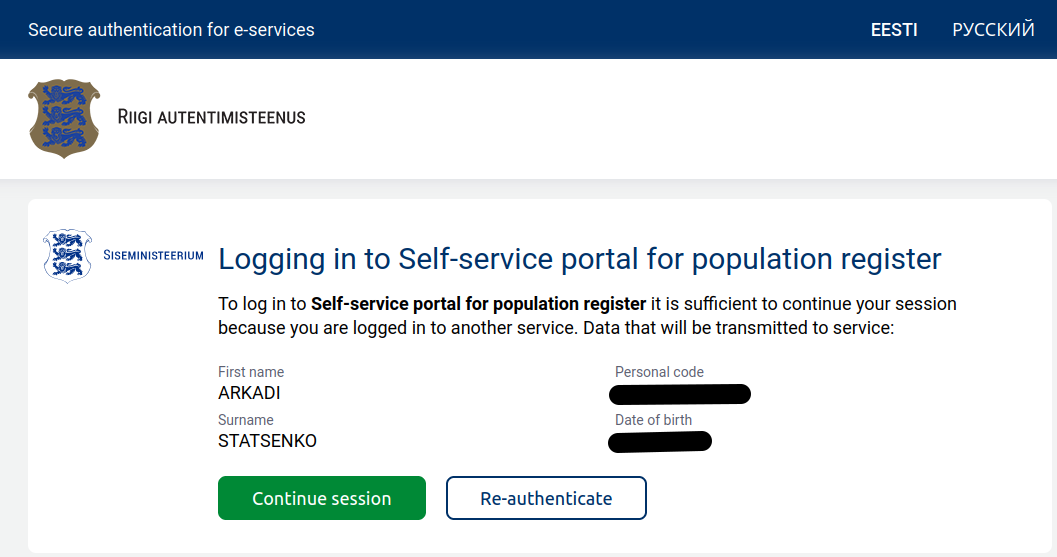
\includegraphics[width=450px]{english/figures/Screenshot from 2025-08-08 20-37-42.png}
\caption{GovSSO single sign-on interface with session continuation option \cite{eesti-ee-screenshot}}
\label{fig:eesti-ee-continue-session}
\end{figure}

However, after experimenting with this method, it was discovered that the 12-hour limitation applies to a different token than initially expected. The time validation is not performed on the client-side JWT token that the application receives, but rather on a server-side master JWT token that is created during the initial \textit{TARA} authentication process (ID-card, Mobile-ID, Smart-ID, etc.) and managed by \textit{GovSSO}.

When a user logs into additional services using the single-sign-on functionality, these secondary sessions are all linked to the same original server-side JWT token managed by \textit{GovSSO}. This architecture means that regardless of which session extension method is used, the 12-hour limit cannot be circumvented because all sessions share the same underlying authentication token that expires after 12 hours.

This limitation has significant implications for the notification system's reliability. Users who expect continuous monitoring must re-authenticate manually at least once every 12 hours to maintain the service functionality. However, this constraint is substantially mitigated by the API's design, which ensures that no data access events are permanently lost, though it does introduce periodic interruptions in real-time monitoring.

Specifically, the API returns comprehensive historical access logs, ensuring that once a user re-authenticates after a session expiry, they will receive all notifications for events that occurred during the period when they were logged out. This behavior is crucial for maintaining data completeness and ensuring that no critical access events are missed due to authentication gaps. The technical implementation of this log handling is detailed in \ref{log-handling}.

Additionally, in order to enhance user awareness of session expiry, the application implements a proactive notification mechanism, as shown in Figure~\ref{fig:session-expiry-notification}, informing the user that they have been logged out and prompting them to re-authenticate to continue monitoring.

\begin{figure}[H]
\centering

\includegraphics[width=250px]{english/figures/Screenshot_20250812_212624_Data Access Notifier.jpg}
\caption{Notification informing the user about session expiry.}
\label{fig:session-expiry-notification}
\end{figure}

\subsubsection{Handling logs and notification delivery}
\label{log-handling}
In this section the following aspects of access log handling will be tackled: their storage, deduplication and filtering.

First of all, user inquiries about themselves are also considered data access and therefore produce access logs. This includes \textit{Andmejälgija} data queries. However, making frequent queries to the \textit{Andmejälgija} API produces numerous logs. 

This makes it important to distinguish logs made by the user themselves from the logs made by third-parties. Thankfully, the \texttt{receiver} field contains the user's Estonian personal code in case the query is made by them. In fact, filtering by whether the receiver field contains user's personal code is exactly how the access log filtering is implemented on \textit{\href{https://www.eesti.ee}{eesti.ee}} itself when the user ticks the ``Exclude queries I have made/initiated" checkbox. Here is the \textit{\href{https://www.eesti.ee}{eesti.ee}} code extract that demonstrates this approach \cite{eesti-ee-portal}:

\begin{listing}[H]
\begin{minted}{javascript}
this.accountService.getUserInfo().subscribe((o) => {
    this.filteredData.data = this.filteredData.data.filter(
        (d) => !d.receiver.toUpperCase()
                   .includes(o.personalCode.replace(/^EE/, ""))
    );
})
\end{minted}
\caption{Estonian state portal JavaScript code for filtering self-access events}
\label{lst:eesti-ee-filtering}
\end{listing}

The same approach was used to implement access log filtering in the \textbf{Data Access Notifier} application. The user's personal code that is needed for filtering is extracted from the JWT token, along with the user's first name which is used to greet the user.

For deduplication of access logs, the \texttt{Set} data structure was utilized. Each access log entry is represented as a data class, and a \texttt{Set} of these entries is maintained to ensure that duplicate logs are not stored or processed multiple times. This approach leverages the fact that \texttt{Set}s in Kotlin do not allow duplicate elements.

To persist the access logs across application restarts and device reboots, Proto Data Store was used, which is Android's recommended solution for storing typed objects or lists in a transactional and type-safe manner. Proto Data Store uses Protocol Buffers \cite{protocol-buffers} for serialization, offering efficient storage and schema evolution capabilities.

Whenever new logs are fetched from the API, they are first filtered to exclude self-access events. The newly fetched logs are then merged with the existing logs stored in Proto Data Store, and the combined set is deduplicated using Kotlin's \texttt{Set} data structure. To determine which logs are new and should trigger notifications, the application computes the set difference between the combined deduplicated logs and the previously stored logs. Only the new items resulting from this difference are used to notify the user. This approach ensures that notifications are sent only for genuinely new access events, while avoiding redundant alerts for logs that have already been seen.

\subsection{Software distribution}

The \textbf{Data Access Notifier} application is distributed as an open-source project hosted on GitHub \cite{data-access-notifier}. Users can download the \texttt{APK} file directly from the GitHub Releases page \cite{data-access-notifier-releases}. To keep the application up to date, users can utilize third-party applications such as Obtainium \cite{obtainium}, which enables automatic updates for applications distributed outside of traditional application stores.

While the application is not currently available from application stores like Google Play Store, this possibility is not excluded in the future. Any updates regarding the application distribution would be posted on GitHub README.

\subsection{User guide}
After installation and opening for the first time, the \textbf{Data Access Notifier} application will prompt the user for necessary permissions, which are the ability to schedule alarms (for AlarmManager to work) as well as to post notifications.

Once the necessary permissions are given, the Log In screen appears. When the Log In button is pressed, an Android WebView is opened, redirecting the user to the \textit{TARA} Log In screen. There the user is free to choose their preferred state authentication option.

The setup process is now complete. As soon as authentication is successfully completed, the user will start receiving notifications whenever new data access logs are returned from the server. There is also a view inside of the application showing all data access logs saved. The setup process is illustrated in Figure~\ref{fig:app-usage}, with the relevant settings page for permitting the application to schedule alarms being opened automatically.

\begin{figure}[H]
\centering
\begin{minipage}{0.32\textwidth}
    \centering
    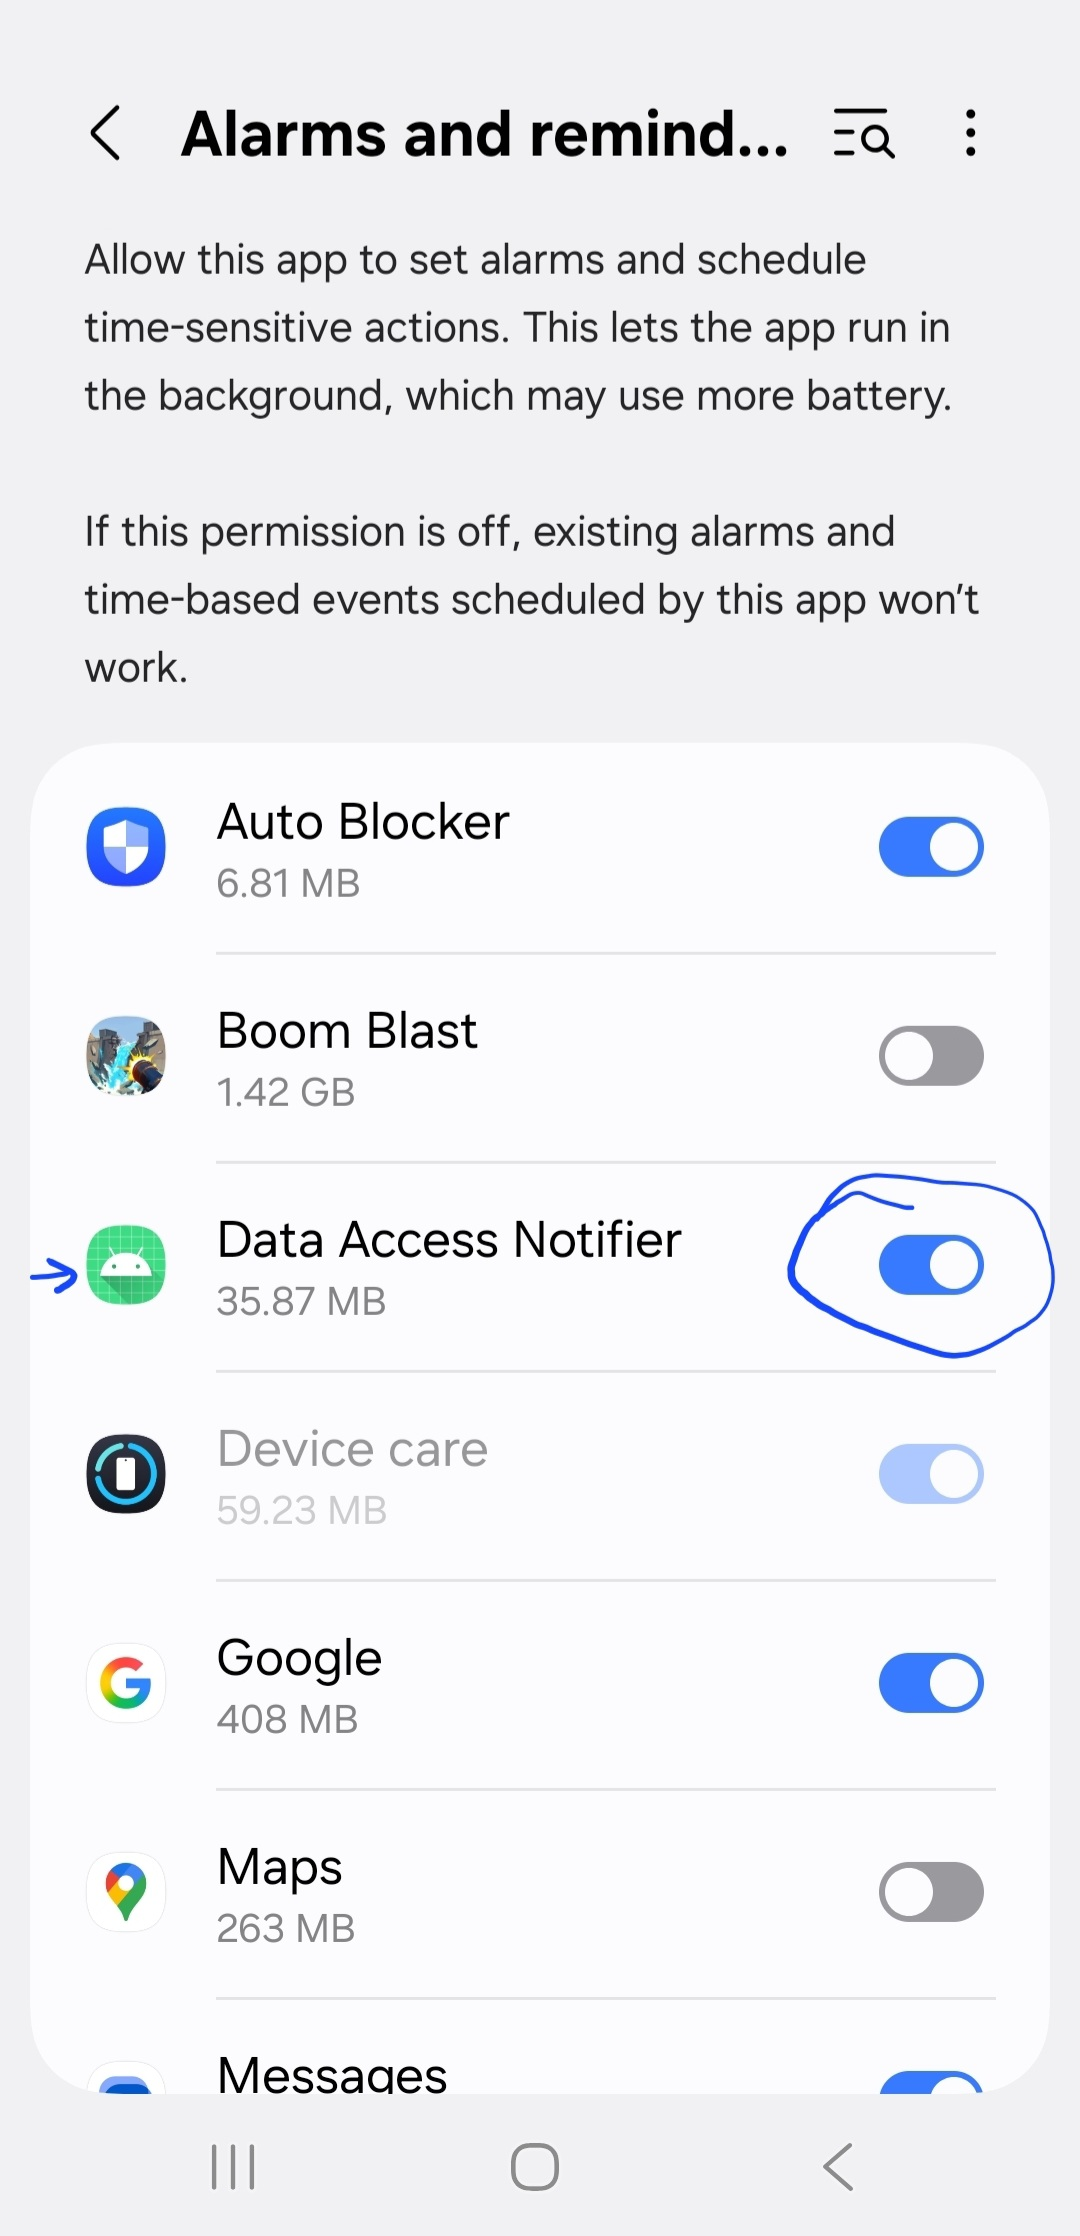
\includegraphics[width=\textwidth]{english/figures/Screenshot_20250812_212139_Settings.jpg}
\end{minipage}%
\hfill
\begin{minipage}{0.32\textwidth}
    \centering
    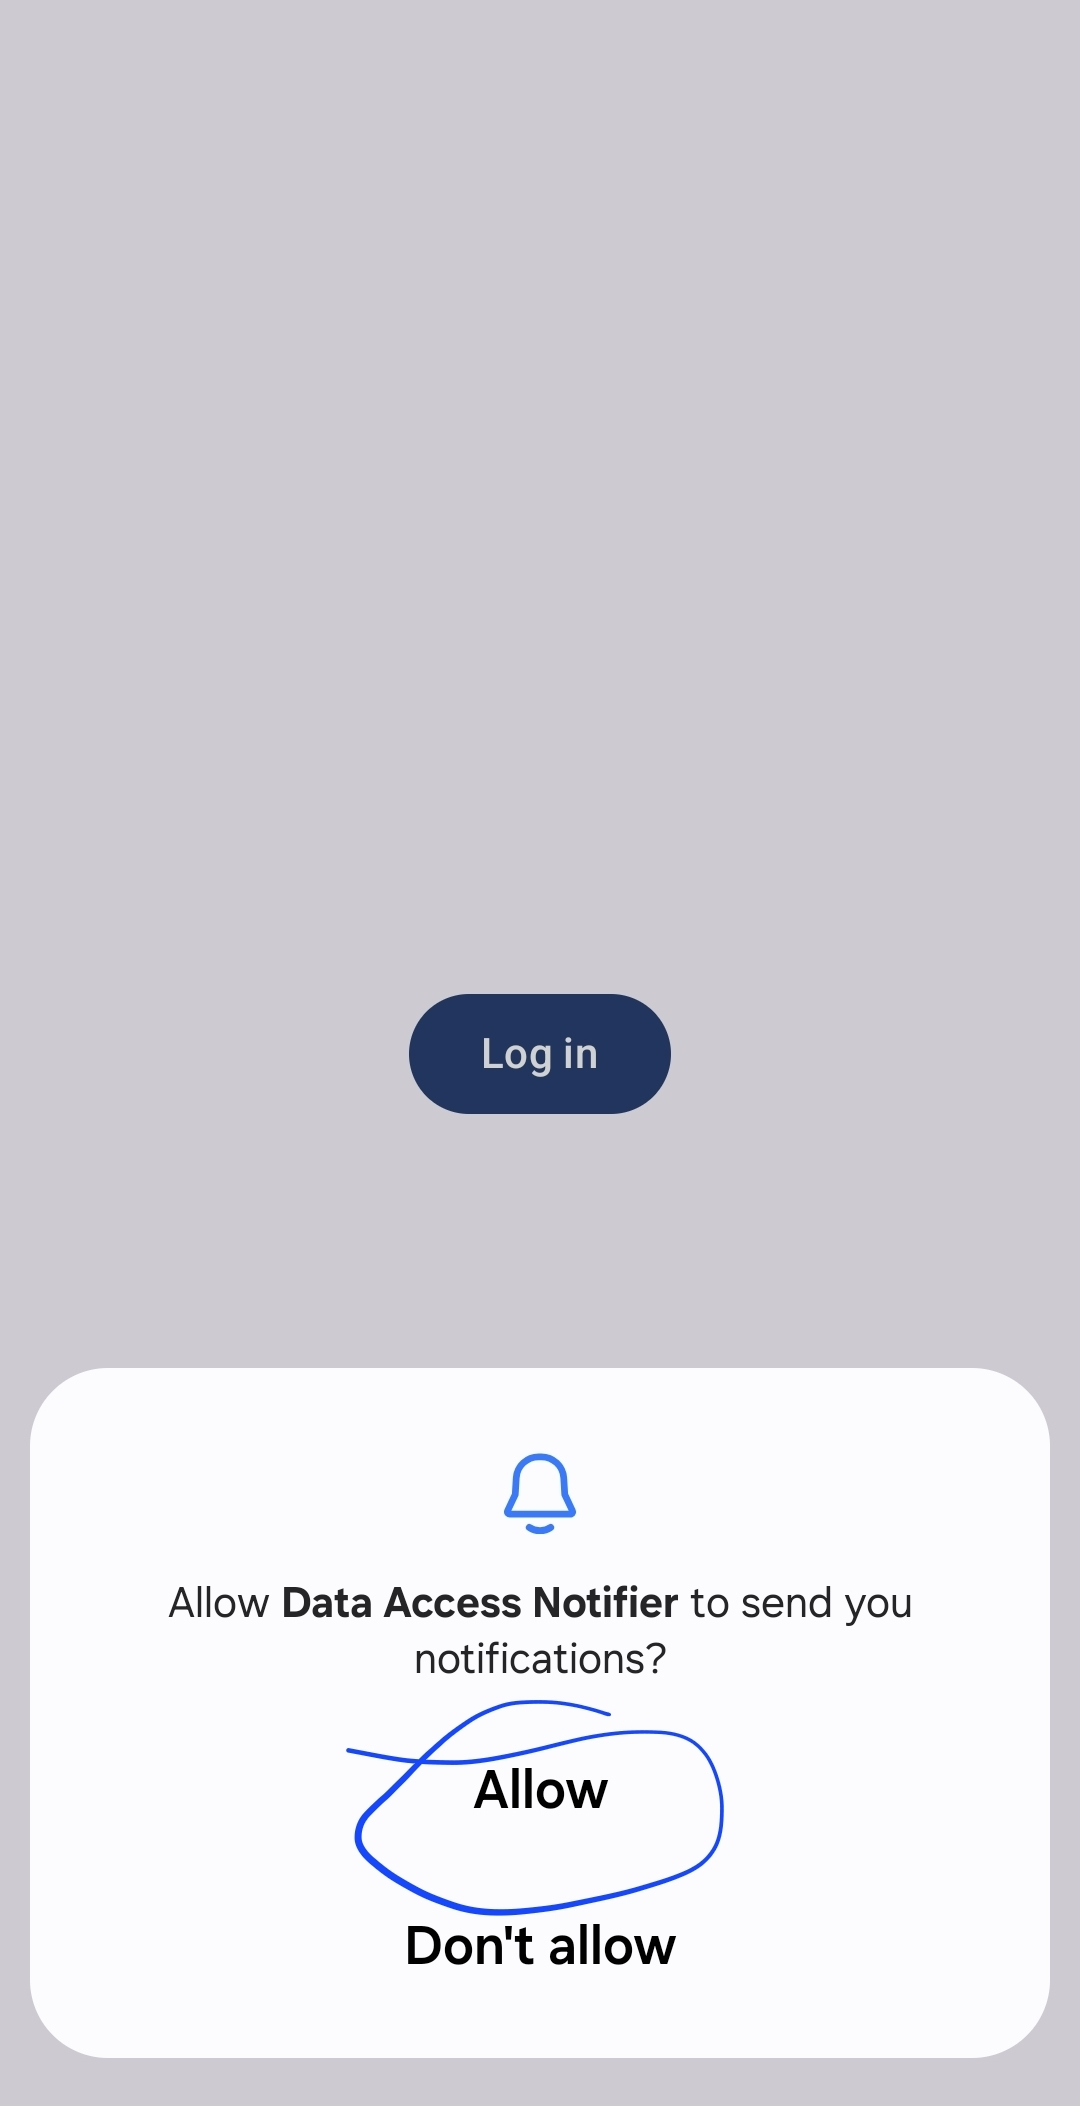
\includegraphics[width=\textwidth]{english/figures/Screenshot_20250812_212153_Permission controller.jpg}
\end{minipage}%
\hfill
\begin{minipage}{0.32\textwidth}
    \centering
    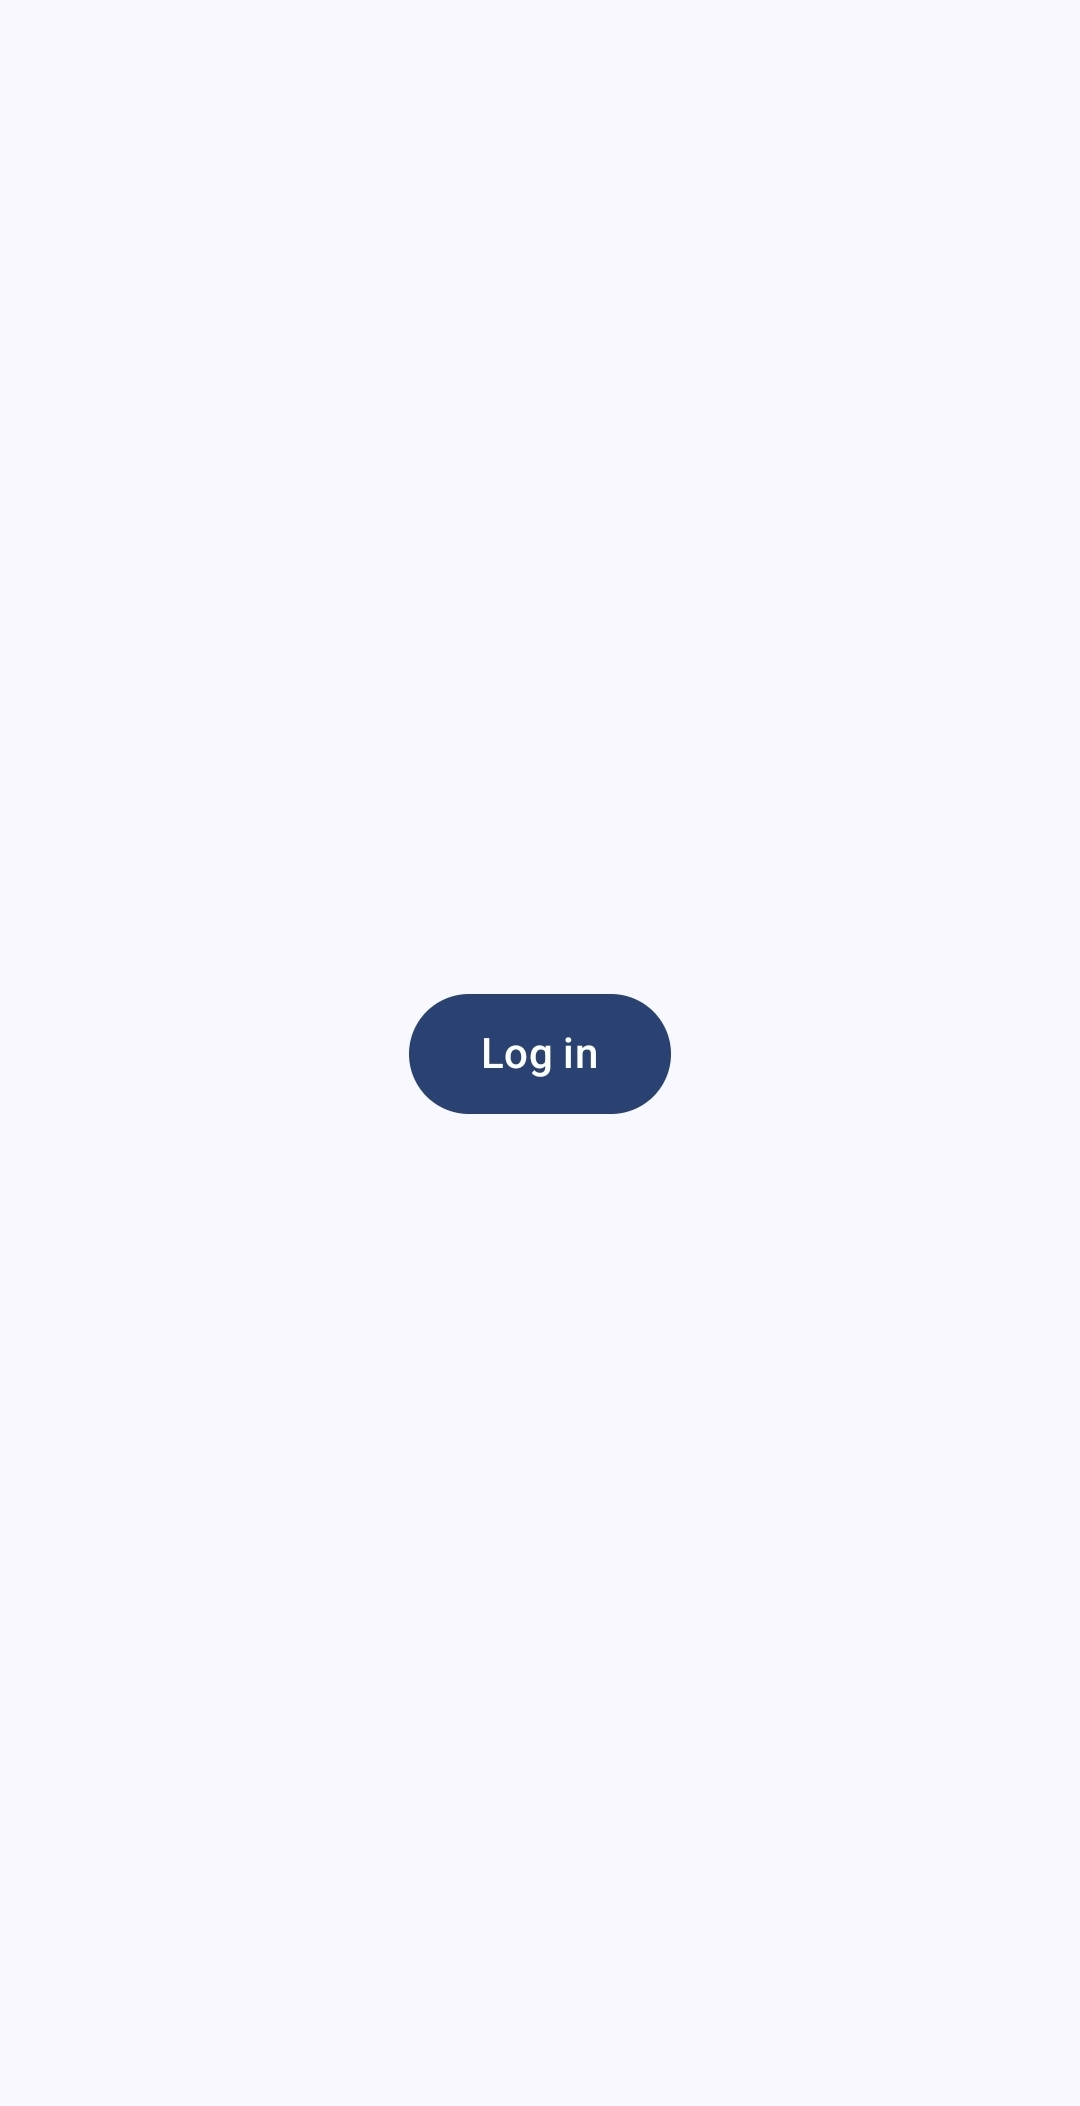
\includegraphics[width=\textwidth]{english/figures/Screenshot_20250812_212555_Data Access Notifier.jpg}
\end{minipage}
\begin{minipage}{0.32\textwidth}
    \centering
    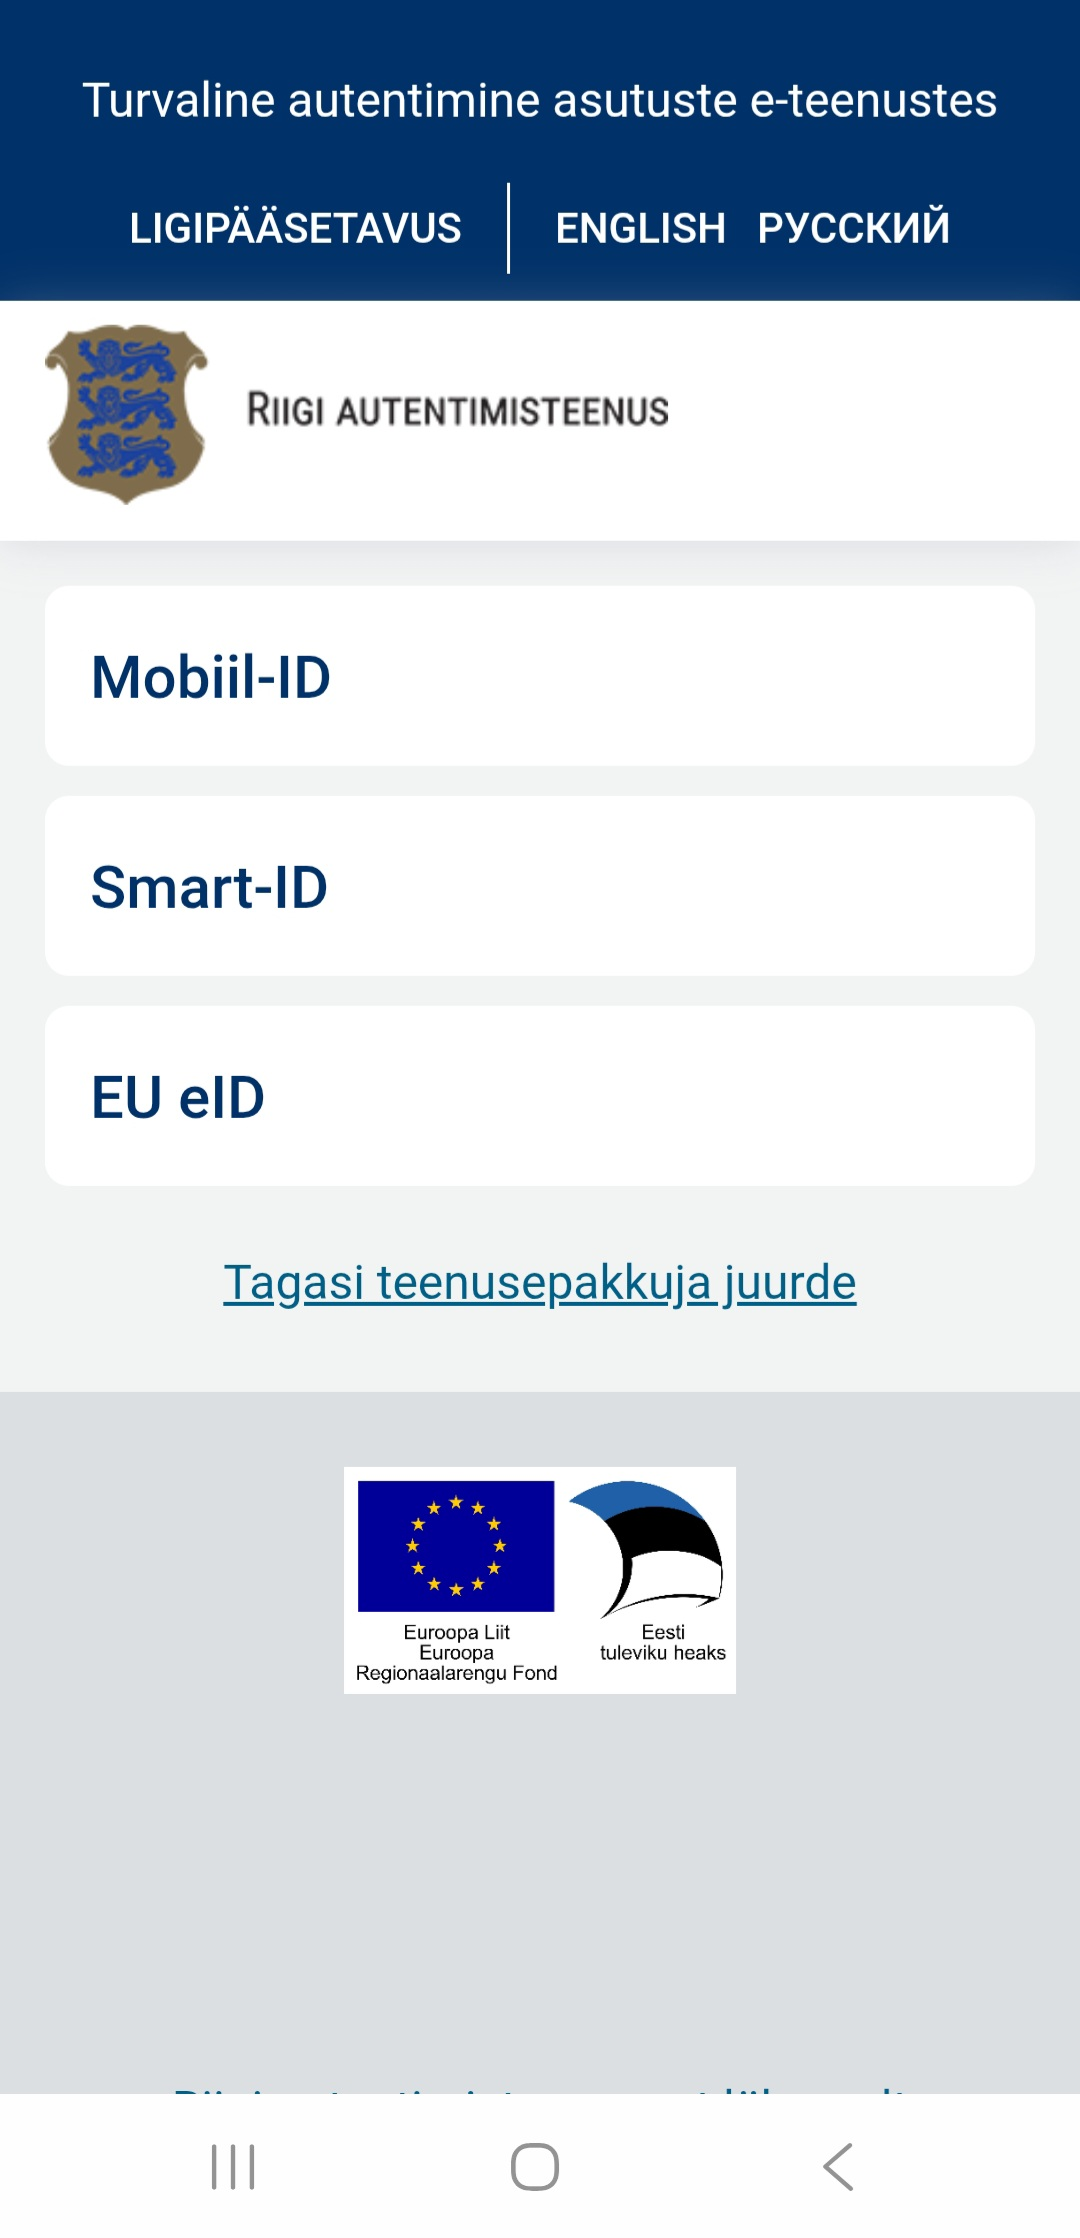
\includegraphics[width=\textwidth]{english/figures/Screenshot_20250812_212238_Data Access Notifier.jpg}
\end{minipage}%
\hfill
\begin{minipage}{0.32\textwidth}
    \centering
    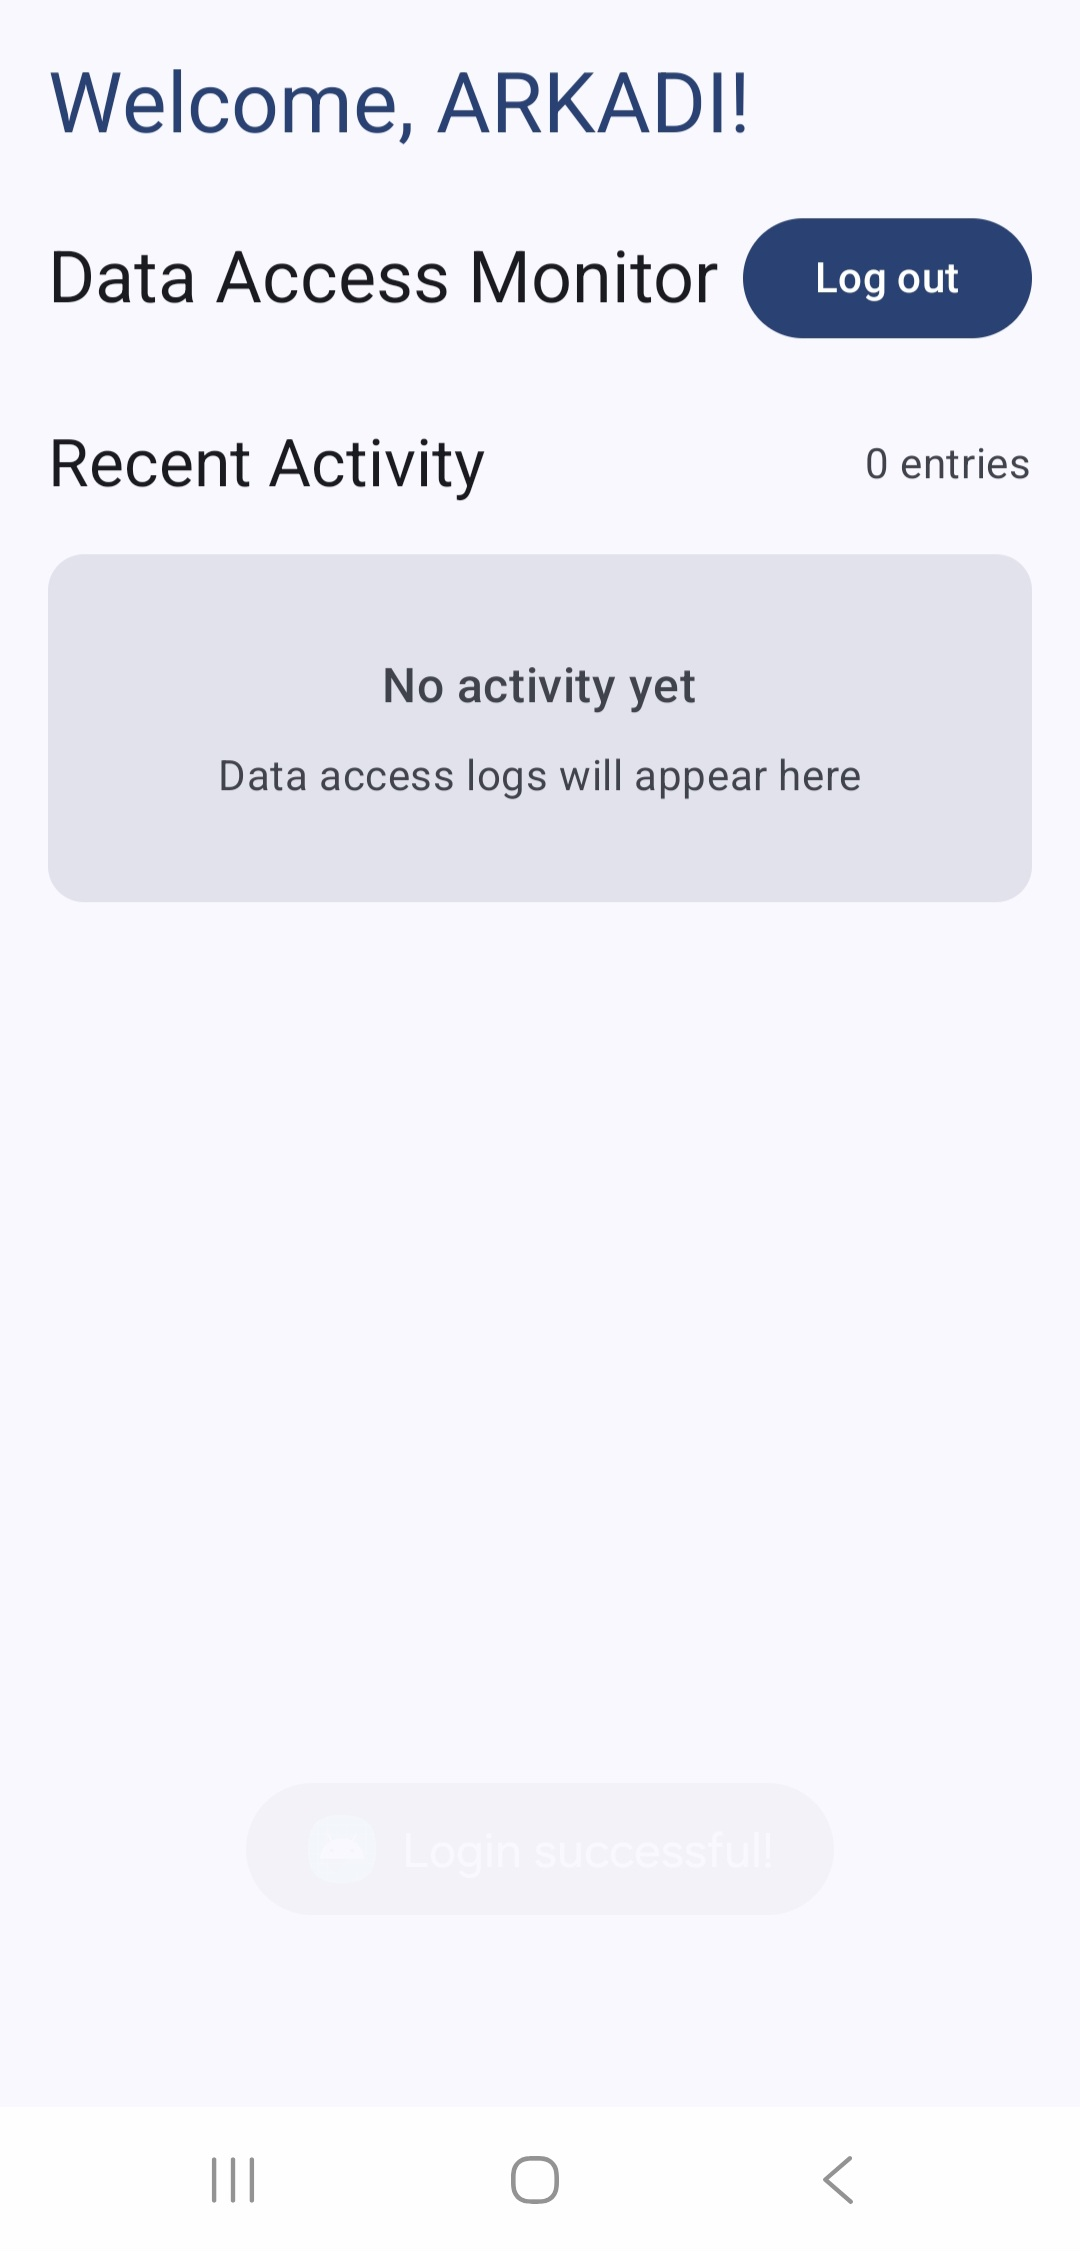
\includegraphics[width=\textwidth]{english/figures/Screenshot_20250812_212306_Data Access Notifier.jpg}
\end{minipage}%
\hfill
\begin{minipage}{0.32\textwidth}
    \centering
    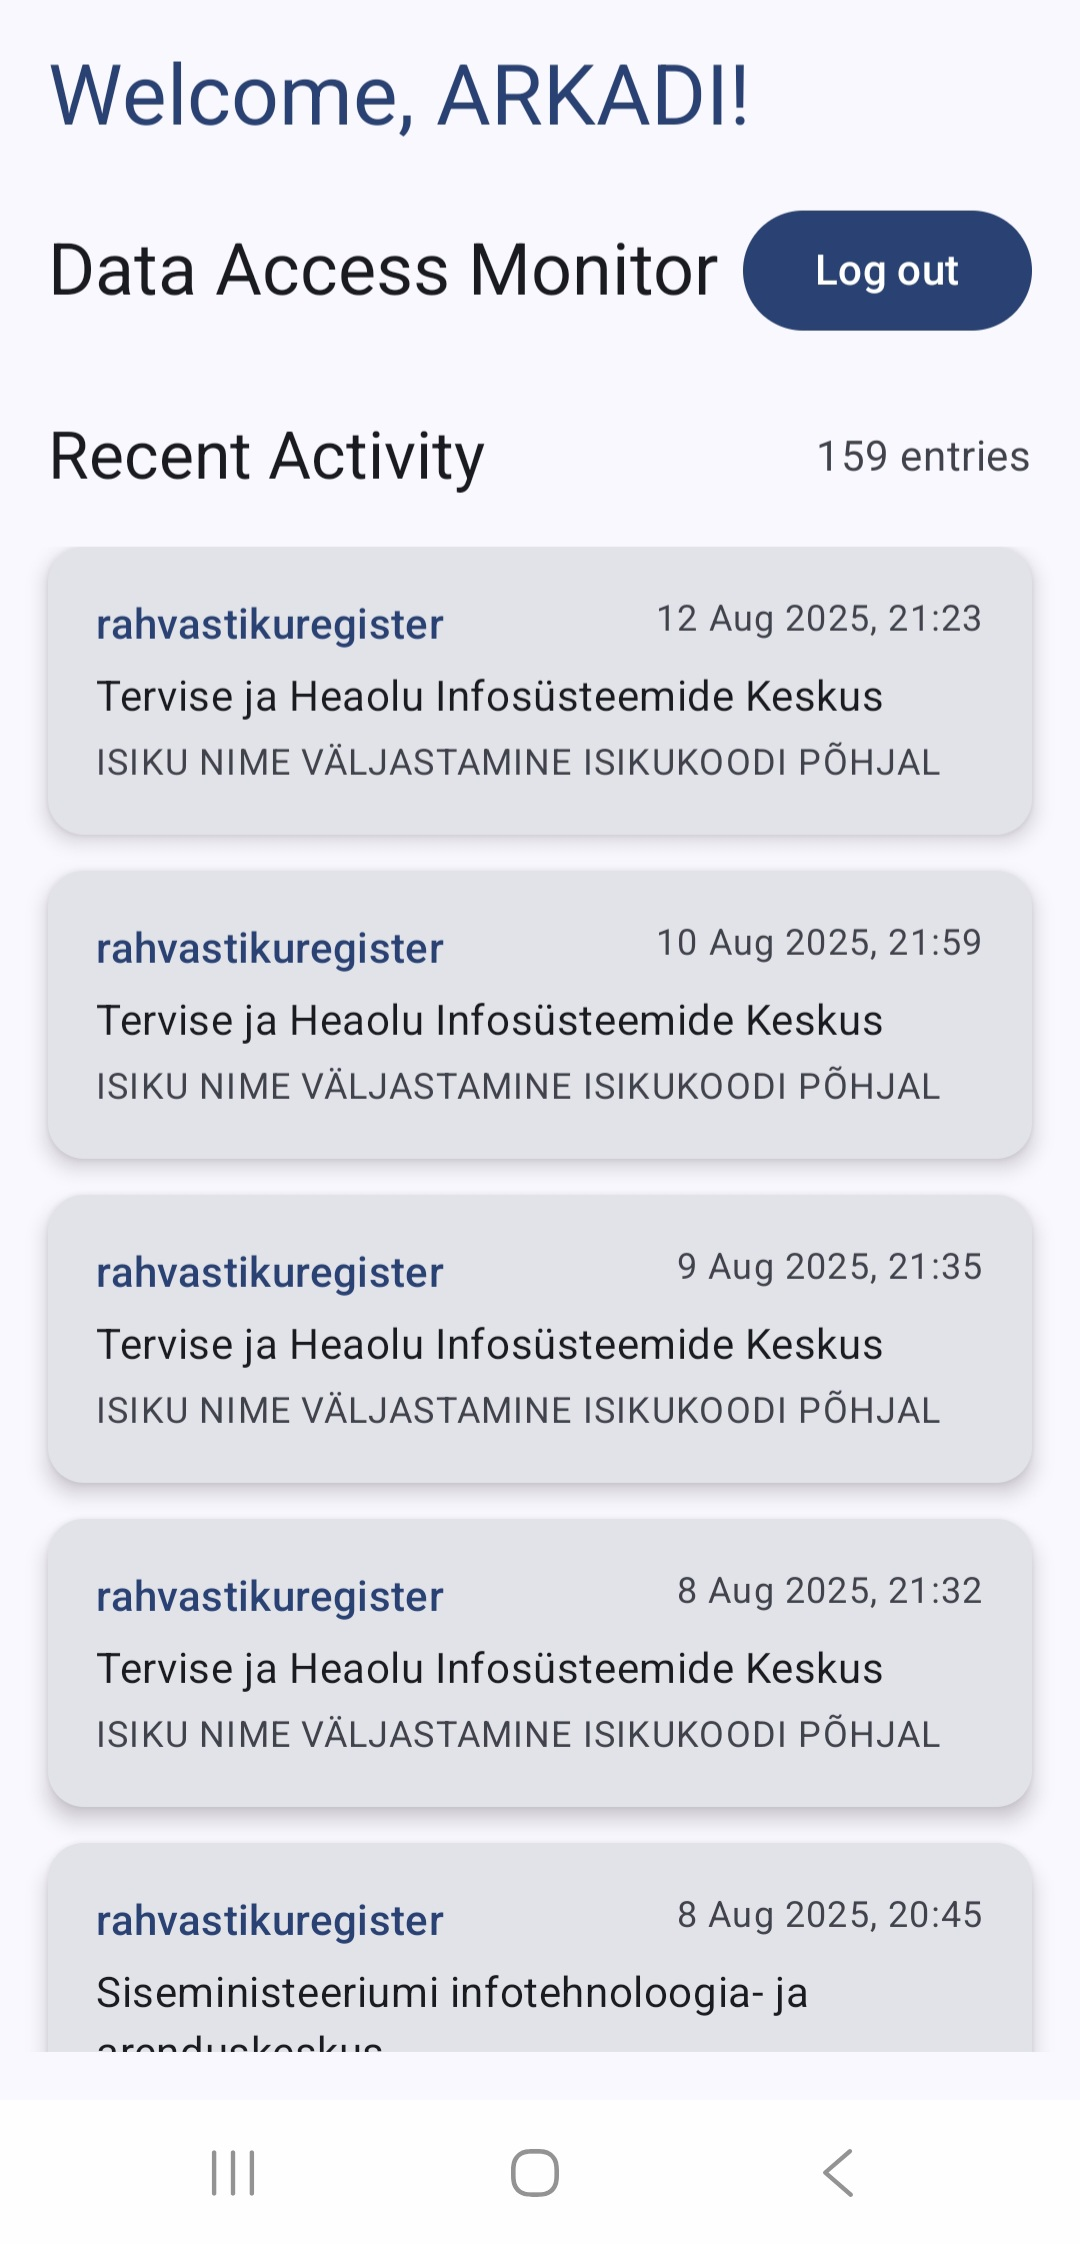
\includegraphics[width=\textwidth]{english/figures/Screenshot_20250812_212336_Data Access Notifier.jpg}
\end{minipage}
\caption{Authentication to Data Access Notifier}
\label{fig:app-usage}
\end{figure} 

Once authenticated, users will start receiving real-time alerts when their data is accessed, as shown in Figure~\ref{fig:data-access-notification}.

\begin{figure}[H]
\centering
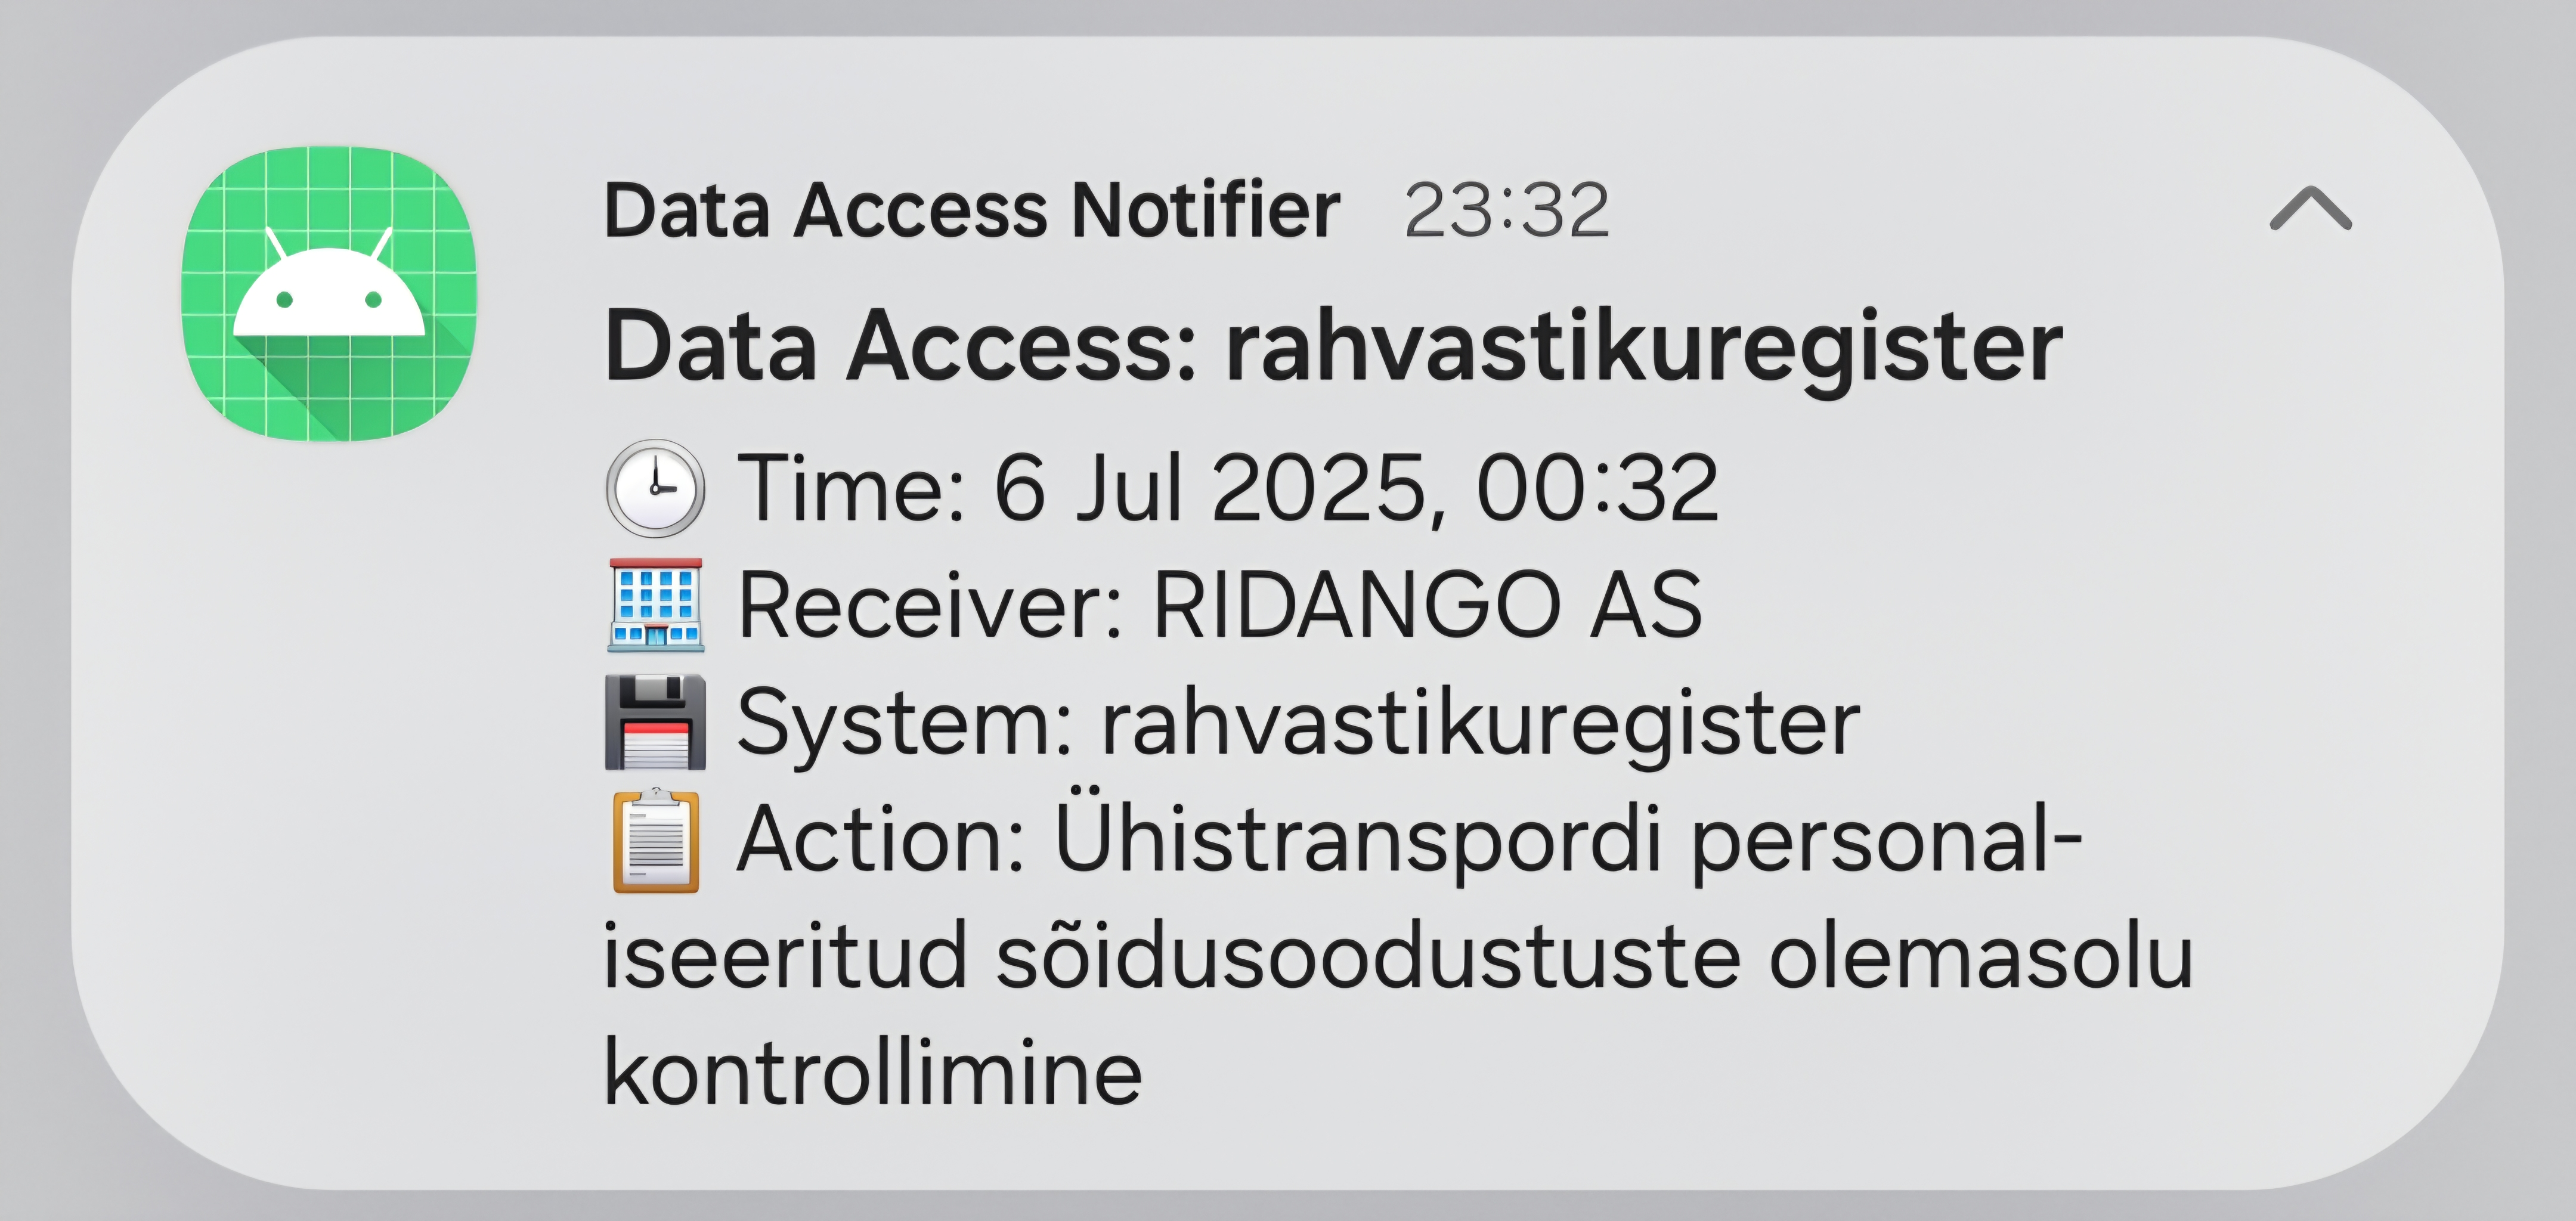
\includegraphics[width=250px]{english/figures/IMG_20250812_233325_272.jpg}
\caption{Data access notification}
\label{fig:data-access-notification}
\end{figure}

\subsection{Observations while using \textbf{Data Access Notifier}}
\label{observations}

While using the \textbf{Data Access Notifier} application over several weeks, several interesting observations were made about the behavior of the \textit{Andmejälgija} API and the reliability of real-time access logging.

One notable discovery was related to delayed log entries. Notifications were occasionally received for access events dated several months in the past - specifically, events from May 2025 would sometimes appear in August 2025. Initially, this was suspected to be a deduplication issue within the application, but after examining the stored notification history, it became clear that these were genuinely new log entries that had not been seen previously by the application.

This behavior suggests that there may be delays in the centralized logging infrastructure of \textit{Andmejälgija}, where some access events are not immediately recorded or made available through the API.

The application demonstrated substantial reliability in maintaining the authentication session during the 12-hour window. The hybrid AlarmManager approach (described in \ref{alarmmanager-approach}) successfully maintained connectivity even during extended periods of device inactivity or network fluctuations.

From a user experience perspective, the notifications provided valuable insights into data access patterns that would otherwise remain unnoticed. This transparency feature proved particularly useful for understanding which organizations access personal data and how frequently such access occurs.

\subsection{Limitations}
The most significant limitation of the \textbf{Data Access Notifier} application is the 12-hour session expiry imposed by the \textit{GovSSO} authentication system. As discussed in \ref{session-limitations}, this server-side restriction cannot be circumvented through known technical means, requiring users to manually re-authenticate.

While the application successfully preserves all access log data during authentication gaps - ensuring no events are permanently lost - the periodic interruptions in real-time monitoring represent a substantial usability constraint.

Additionally, the application's scope is currently limited to Android devices running version 8.1 and higher. While this covers approximately 96.4\% of the Android ecosystem, users of iOS or other mobile platforms cannot benefit from this solution without platform-specific implementations.

The reliance on reverse-engineered internal APIs also introduces inherent fragility. Changes to \textit{\href{https://www.eesti.ee}{eesti.ee}}'s internal API structure or authentication mechanisms could potentially break the application's functionality without notice, requiring an update to the application to fix the issue.

Additionally, the session-based approach requires the device to maintain active network connectivity and remain operational to perform periodic authentication renewals and API polling. Extended periods of device inactivity, airplane mode, or network unavailability will result in session expiry and temporary loss of monitoring capabilities.

The application also doesn't currently support the access logging implemented in \textit{E-File}.

Finally, the \textit{Andmejälgija} protocol itself is not regulated by the law yet, so information systems are not required to implement it, and even if they do, not all data access events are guaranteed to be timely distributed or logged at all.

\subsubsection{Tested devices}
The \textbf{Data Access Notifier} application has been tested on the following devices:
\begin{itemize}
    \item Xiaomi Poco X3 Pro running CrDroid without Google Services 
    \item Xiaomi Redmi 7A running Lineage OS without Google Services
    \item Samsung Galaxy S25 with stock OS (Google Services included)
\end{itemize}

\subsection{Battery usage}
\textbf{Data Access Notifier} application maintains relatively low power consumption despite its continuous background operation. The hybrid AlarmManager approach with short-lived foreground services appears to be efficient in terms of battery impact.

While the battery utilization hasn't been actively monitored, some screenshots have been taken on Samsung Galaxy S25 at different times during the active use period, as shown in Figure~\ref{fig:battery-usage}.

\begin{figure}[H]
\centering
\begin{minipage}{0.32\textwidth}
    \centering
    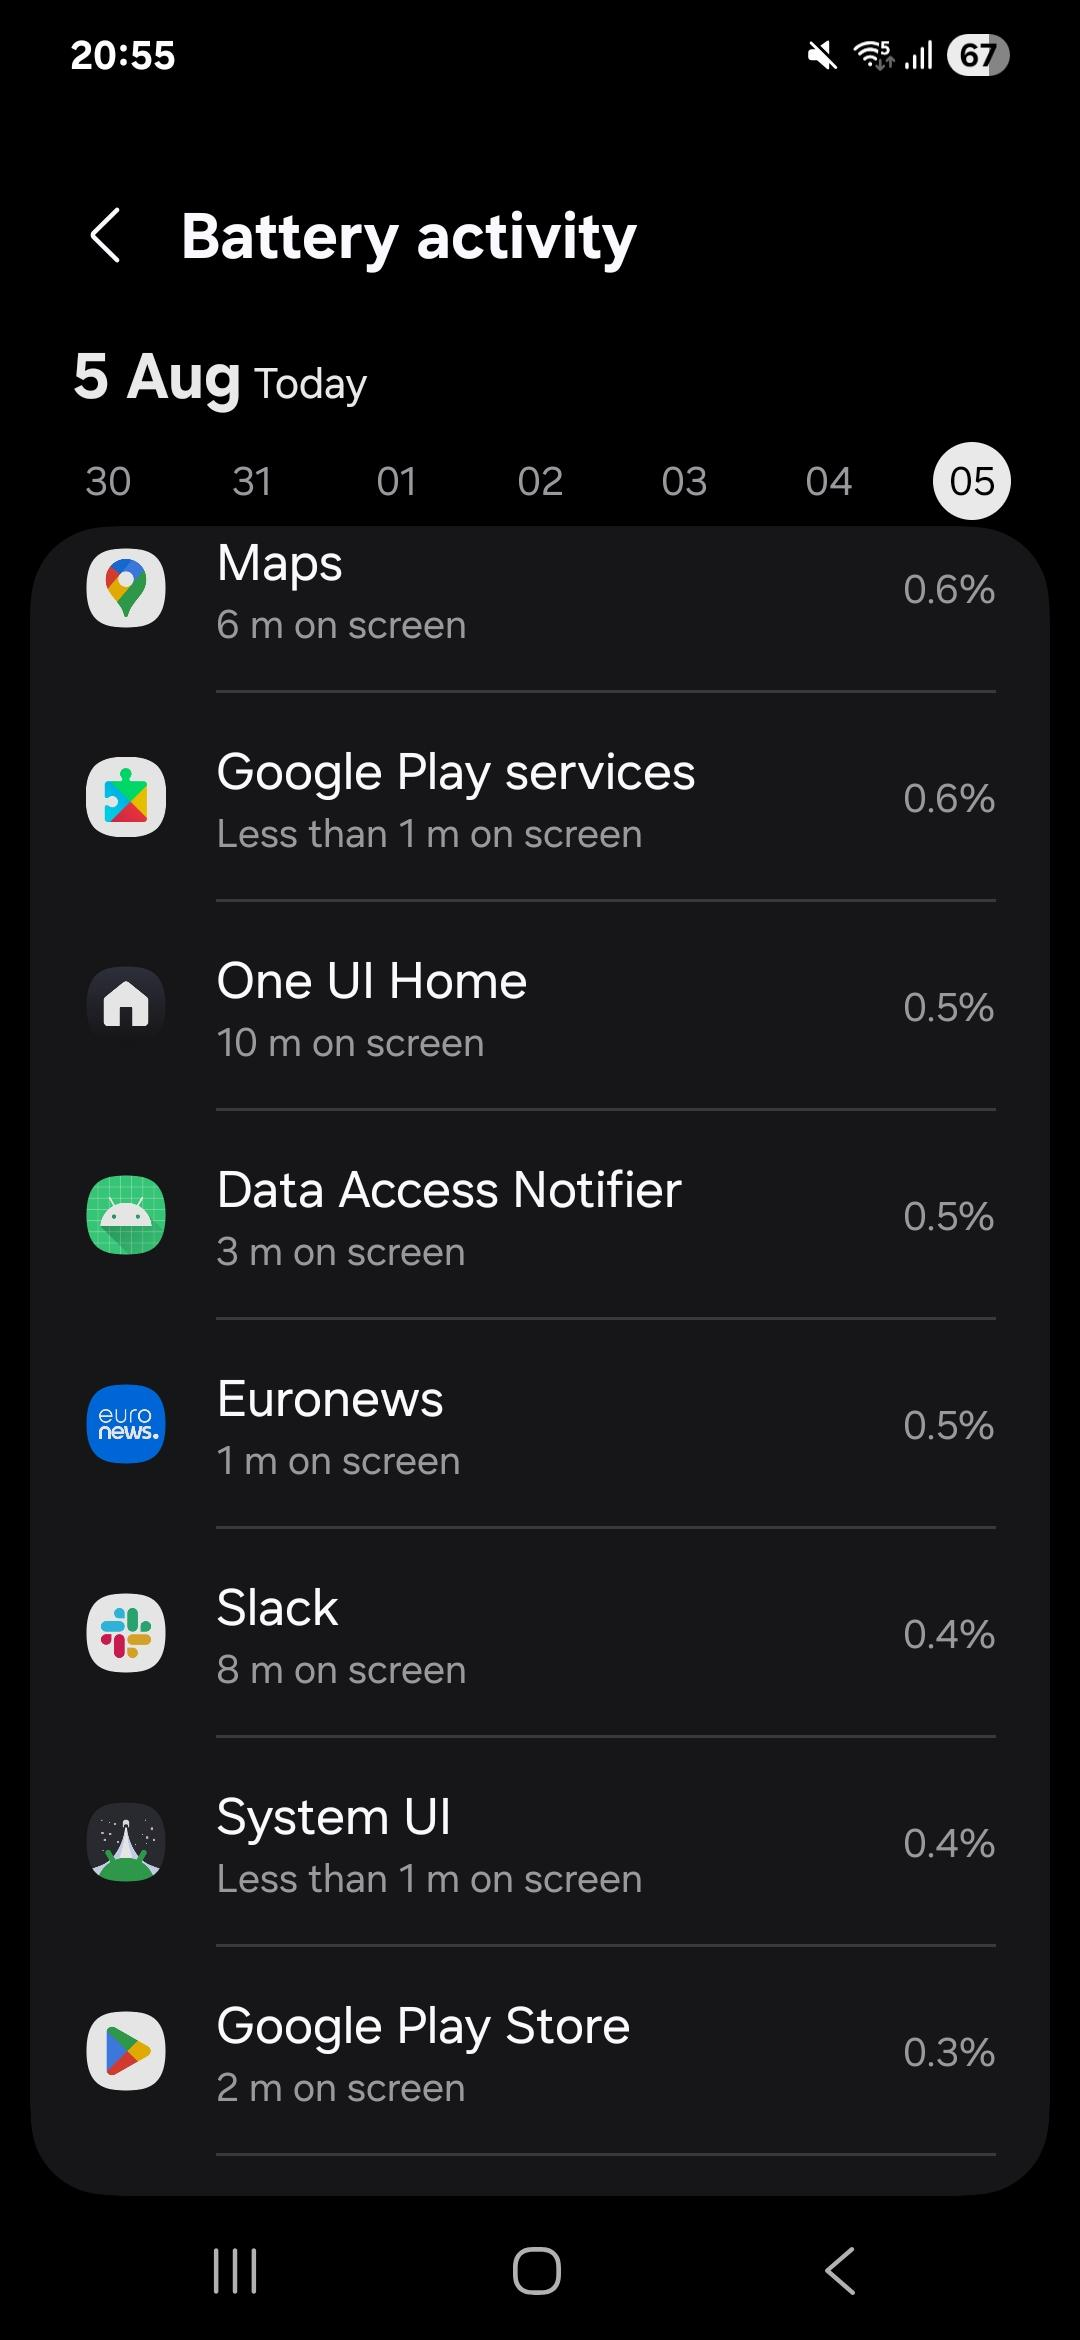
\includegraphics[width=\textwidth]{english/figures/IMG_20250809_225839_242.jpg}
\end{minipage}%
\hfill
\begin{minipage}{0.32\textwidth}
    \centering
    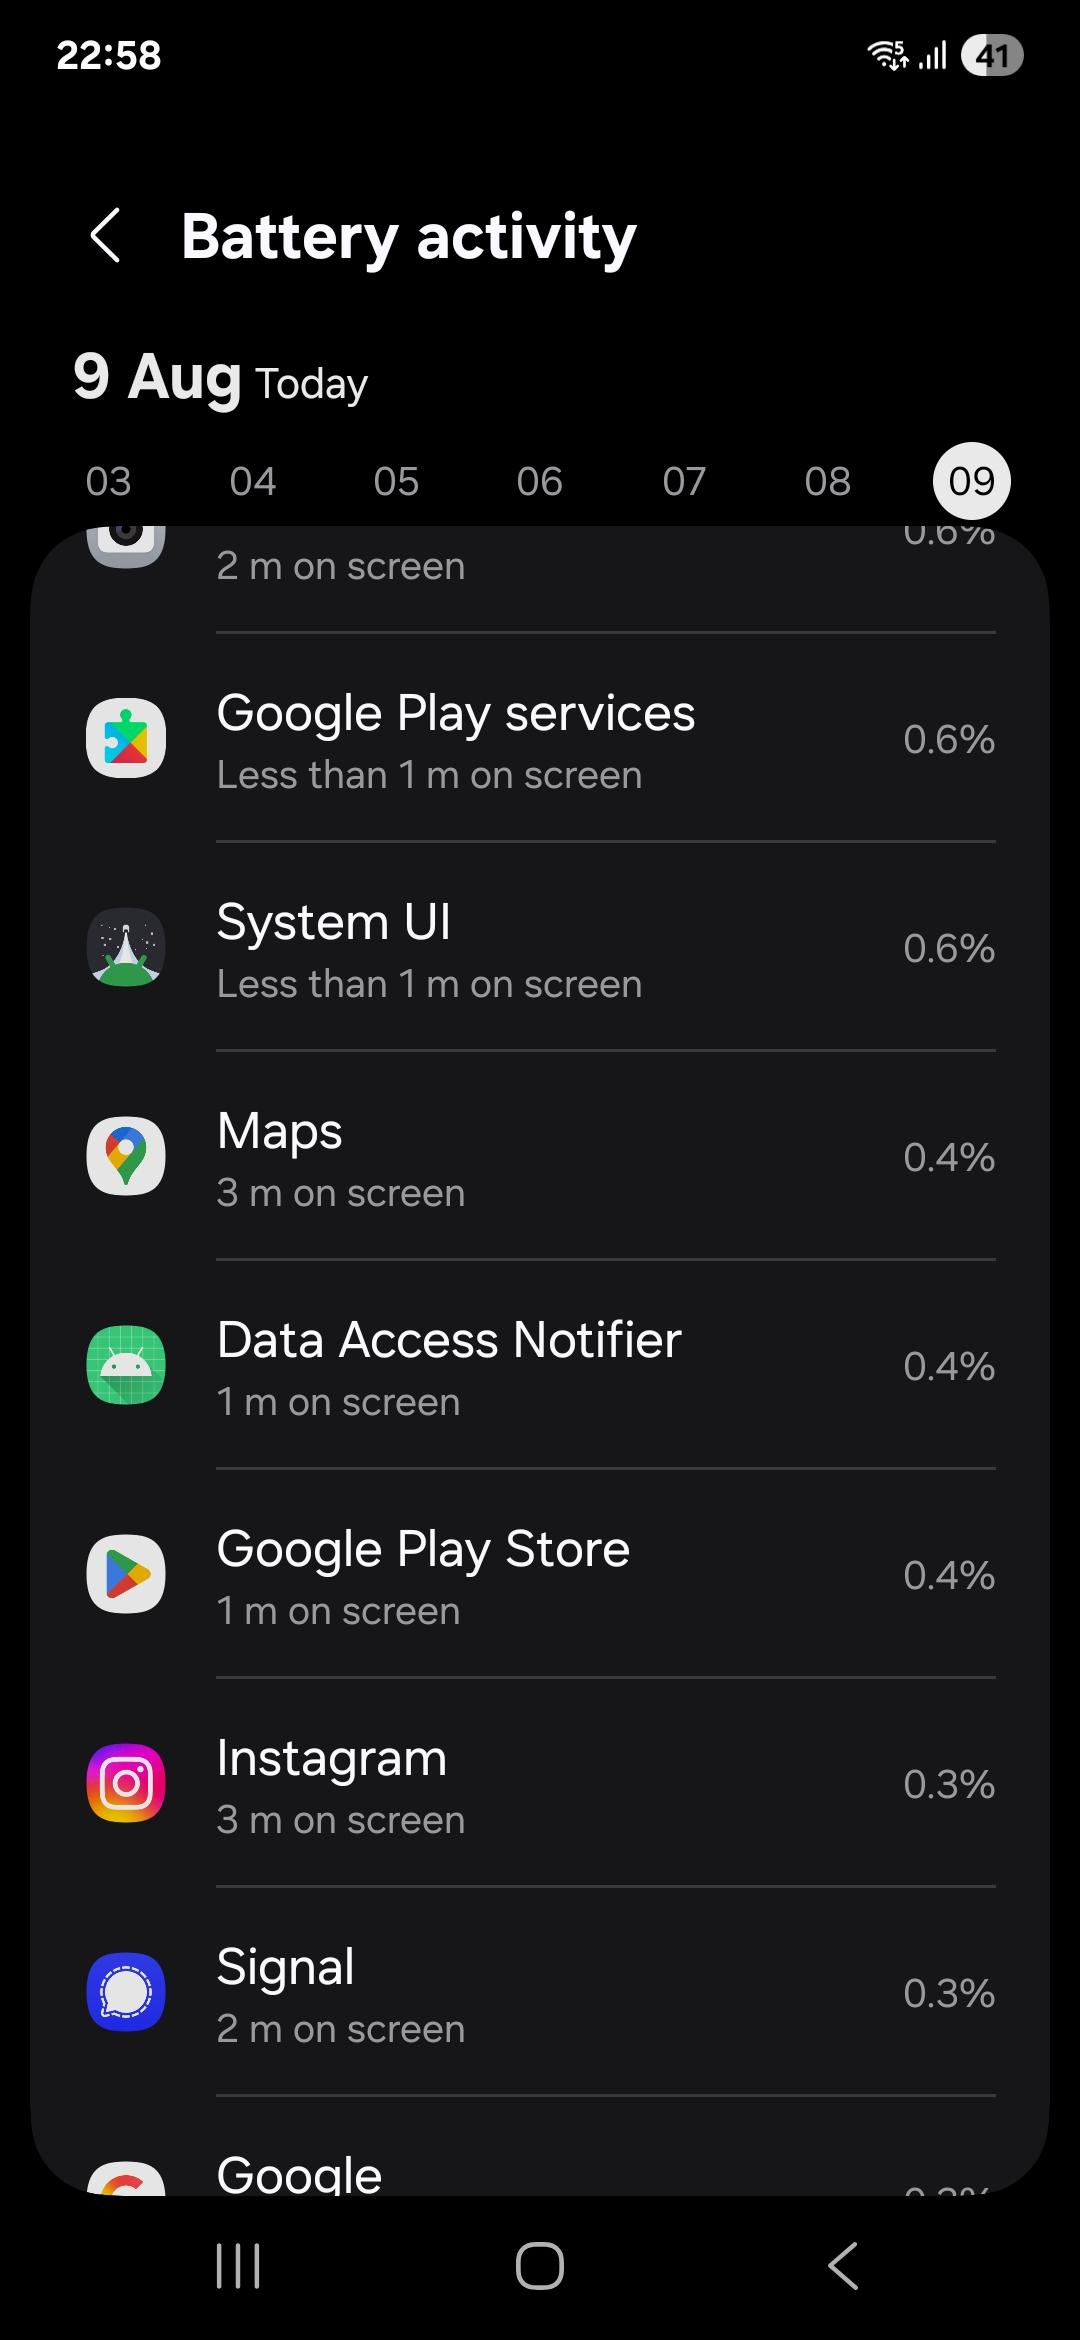
\includegraphics[width=\textwidth]{english/figures/IMG_20250809_225839_290.jpg}
\end{minipage}%
\hfill
\begin{minipage}{0.32\textwidth}
    \centering
    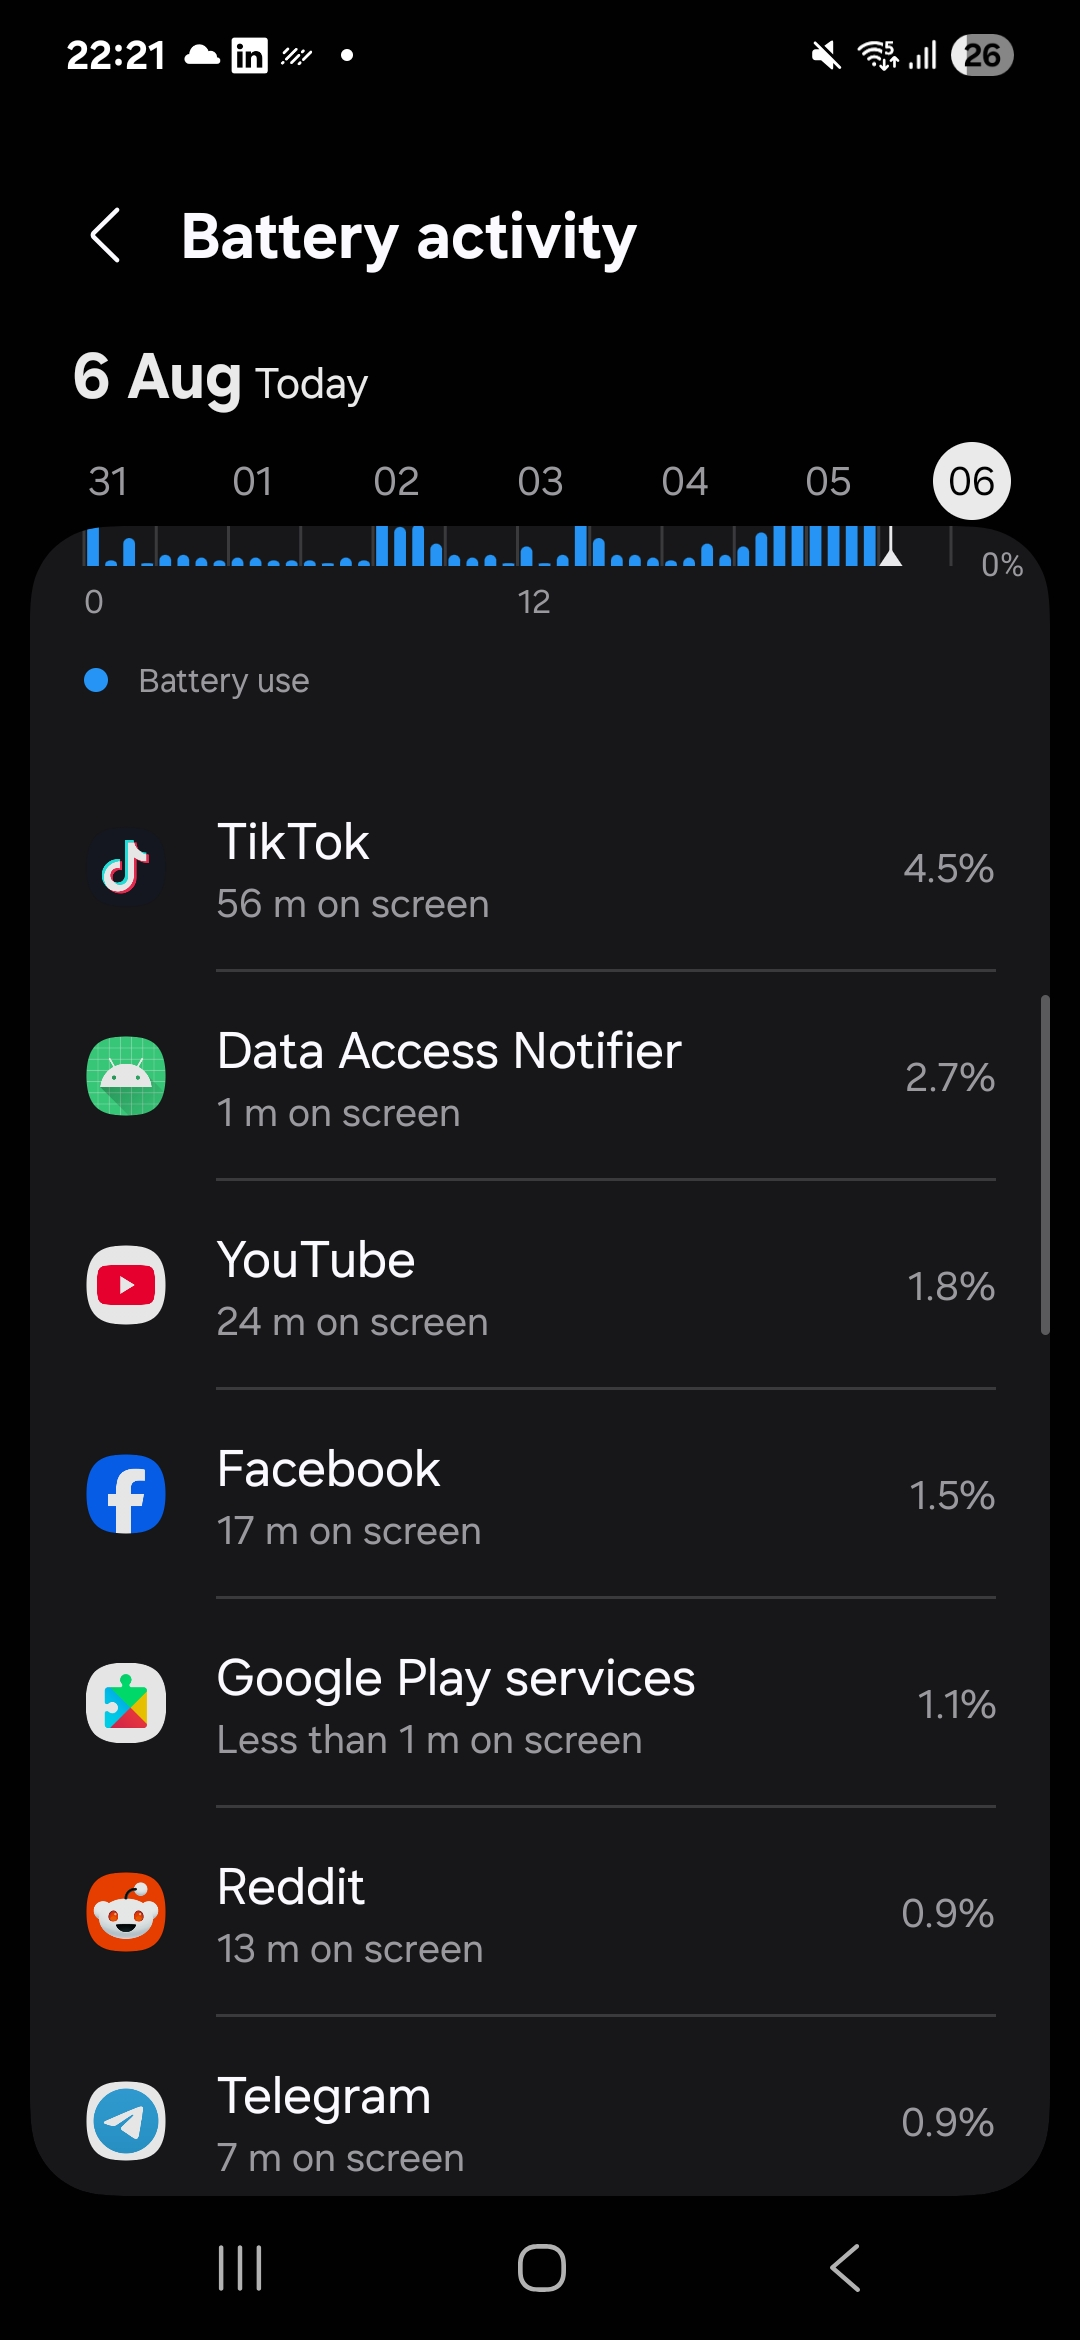
\includegraphics[width=\textwidth]{english/figures/IMG_20250809_225839_295.jpg}
\end{minipage}
\caption{Battery usage statistics for Data Access Notifier on Samsung Galaxy S25}
\label{fig:battery-usage}
\end{figure}

\subsection{Bug reports}

Users are encouraged to report any bugs, issues, or unexpected behavior through the GitHub Issues page of the project repository \cite{data-access-notifier}. When submitting bug reports, users should include:

\begin{itemize}
    \item Device model and Android version
    \item Detailed description of the issue
    \item Steps to reproduce the problem
    \item Any relevant error messages or screenshots
    \item Application version number
\end{itemize}

This feedback mechanism helps improve the application's stability and reliability across different Android devices and configurations.

\subsection{Contributions}
The \textbf{Data Access Notifier} project welcomes contributions from the community. Contributions are to be submitted as pull requests to the GitHub repository. Contributors can also contact the original author directly at \href{mailto:arkadistatsenko@gmail.com}{arkadistatsenko@gmail.com} for questions, suggestions, or collaboration opportunities.





%\section{Formatting}  \label{formatting}
Many different tools, some of which You might not even be aware of, will be used to format Your thesis. As good formatting makes up 25\% of Your thesis grade, it is important to take it seriously and allocate sufficient time. Especially if You have not previously formatted documents of that size that well or learned the use of corresponding tools. This chapter looks at the formatting principles for different parts of the thesis.

667578801\subsection{The Title and Info Pages}
The very first page – the title page – is already formatted in this template. The title page must include the curriculum You plan to graduate from (including the educational institution and the institute), thesis title, kind and volume corresponding to the level of studies, Your name, the names (and, optionally, the academic degrees) of Your supervisors, publication location, and year. The information that goes to your title page must be entered into the specific fields in the file \path{thesis.tex}. Be sure to check the corresponding information. For example, if You decide to add the academic degrees of Your supervisors, check if an abbreviation is MSc (Master of Science) or MA (Master of Arts). The degrees differ depending on the curricula.

The info page (file \path{0-info.tex}), which follows Your title page, includes the abstract, keywords, and CERCS codes of Your work. The abstract should give an overview of everything done during Your work. For example, if three of Your content chapters thoroughly describe the different processes and results of Your work, then that should be readable from Your abstract. Concentrate on mentioning in the abstract what You did that can be read about in the thesis.

Keywords are the different terms and names that designate important aspects of Your work. To come up with keywords, You should think about Your work generally. What important terms come to Your mind if You think about Your work as a whole? For inspiration, it is good to check out the keywords of previous theses made on similar topics. Joonis~\ref{fig:keywords} shows the word cloud of keywords from the theses defended at the Institute of Computer Science in 2015–2020\footnote{\url{https://cglearn.eu/theses/top}}.

\begin{figure}[ht]
    \centering
    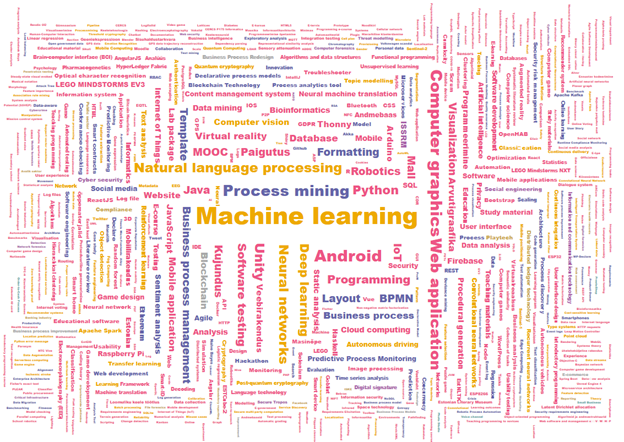
\includegraphics[width=\textwidth]{figures/Figure1-Keywords.png}
    \caption{The word cloud of keywords from theses defended at the Institute of Computer Science in 2015–2020.}
    \label{fig:keywords}
\end{figure}

Besides the keywords, You also need to assign a Common European Research Classification Scheme (CERCS) code to Your work. These codes classify research areas. Often, it can be hard to classify a thesis using a specific classifier. Still, You must find a classifier that Your work fits under the best. You can use several CERCS codes. The classifiers are on the Estonian Research Information System’s web page: \url{https://www.etis.ee/Portal/Classifiers/Index/26}.

After the info page, You can also add a visual abstract to Your work. That will be a single figure that efficiently describes the process and results of Your work. The figure has to include the information listed in the Guidelines for preparing and grading of graduation theses at the Institute of Computer Science of the University of Tartu document. When using the institute’s logo, respect its protected area – it must have the height of the house of free space around it. The visual abstract is helpful to add, as it quickly conveys the nature of Your work to the reader. You can reuse the graphics later on Your defense slides and when popularizing Your work.

\subsection{Structure}
It is essential for the reader of Your work that Your document is structured logically and clearly. Good titles and reasonable content sectioning to chapters and sub-chapters guide the reader through Your thesis.

\subsubsection{Titles}
Both the thesis title itself and the chapter titles should be concise and on-point. Long titles could carry too many ideas within themselves, and You can lose Your reader already at the title. The main title of the thesis should maximally fit on two lines.

In English, the words in titles start with capital letters. There are different styles, but generally, all the words besides pronouns should start with a capital letter. It is good to use the Capitalize My Title tool: \url{https://capitalizemytitle.com/}

In Estonian, however, only the very first letter of the title is capitalized, and the rest of the words are written just like regularly.

Punctuation should be avoided in titles. Depending on the nature of Your work, an em or en dash could be reasonable. For example, if You have created a software product, it is good to mention the product's name in the title, followed by a longer dash and a description of its unique value. On the other hand, a sentence with commas or question marks would not fit as a title.

These principles also apply to the titles of Your chapters, which are called headings. The content chapter headings start with numbers. It is up to You if You start the numbering from the Introduction chapter and end it with the Conclusion chapter or leave these two chapters unnumbered. In this template, the Introduction and Conclusion chapters are also numbered. The Conclusion chapter is followed by unnumbered sections called References and Appendices. For different appendices, it is reasonable to use some numbering again. To number the appendices, You can use Roman numerals (Appendix I, Appendix II) or capital letters (Appendix A, Appendix B).

The subchapter numbering includes the number from the parent chapter. For example, the subchapters of chapter 2 are numbered 2.1, 2.2, etc. The dot mark after the entire numbering is used only in the first-level headings. Starting from the third-level headings, the numbering can be omitted. In this template, the heading styles (\verb|\section{...}|, \verb|\subsection{...}|, etc) provide the correct numbering.

\subsubsection{Table of Contents}
At the beginning of Your work, after the info page and visual summary, but before the first chapter, there is the Table of Contents. Capable text editing software generates the Table of Contents automatically. In this template, the table of contents is created by the command \verb|\tableofcontents|. That command generates the table of contents automatically based on the sections/headings (\verb|\section{...}|, \verb|\subsection{...}| jne) of the document.

\subsection{Text}
The alignment of the thesis text must be justified (straight rug from both left and right). Justified alignment can create a situation when the spacing between words in one line is visually too much. In such cases, the line can be hyphenated to fix the visually bothersome spacing. Many text editors have automatic hyphenation capabilities, but these are prone to over-hyphenation. In this template, the automatic hyphenation is minimized and the package \verb|microtype| ensures that the spacing between the words would not get too large. Having hyphenated words hinders the readability of the text, so hyphenation should be used minimally. One should avoid situations when multiple subsequent rows are hyphenated.

The guidelines for preparing and grading of graduation theses at the Institute of Computer Science of the University of Tartu document presents many text formatting rules. For example, the line spacing of text should be in the range 1.0-1.5. This template uses 1.4 line spacing which visually corresponds to the 1.5 line spacing of Microsoft Word.

It is possible to use italics (\verb|\emph{...}|), bold (\verb|\textbf{...}|), or other text formatting tools to emphasize some terms or ideas in Your text. However, it is good to use these tools sparingly so as not to make Your work visually too hectic.

When writing paragraphs, You should observe that there would not be a single lone word at the last row of the paragraph. This is called an orphan word, and it is not visually very good. Checking for orphan words or lines (an orphaned line of text at the beginning of a page that is followed by a new chapter or empty page) is something one should do as one of the last things when formatting their fair copy.

\subsection{Elements}
Many different elements like figures, tables, and code examples improve the appearance and reader’s understanding of Your thesis.

\subsubsection{Figures}
All the different images, be they plots, photographs, or screenshots, are labeled as figures. When adding an image, it should be labeled as a figure, numbered, and captioned. In the LaTeX template here, this is done by first adding or uploading the image to the \verb|figures| folder. Afterward the image can be used via the following code:

\begin{minted}[escapeinside=||]{tex}
\begin{figure}
    \centering
    \includegraphics[width=\textwidth]{figures/|\textbf{Figure1-Name.png}|}
    \caption{|\textbf{Figure caption text.}|}
    \label{fig:|\textbf{figureLabel}|}
\end{figure}
\end{minted}

The code above must include the correct file name with the file extension inside the \verb|figures| folder, a short caption text, and a short \emph{label} for cross-referencing the figure.

It should be clear from the caption what is depicted in the image. The caption is shown under the figure together with the element's label \emph{Figure} and an automatic number.

\begin{wrapfigure}{r}{0.33\textwidth}
    \centering
    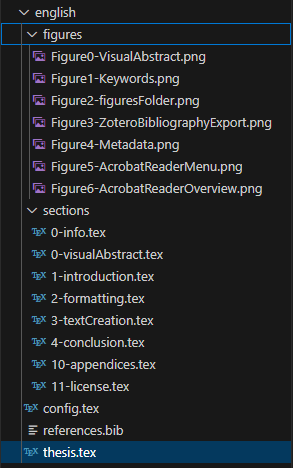
\includegraphics[width=0.33\textwidth]{figures/Figure2-figuresFolder.png}
    \caption{Template folders.}
    \label{fig:folders}
\end{wrapfigure}

You can add the images in the middle of the page or wrap text around them. To add a figure that is wrapped by text, write \verb|wrapfigure| instead of \verb|figure| in the example above. The figure's width could be, for example, \verb|width=0.33\textwidth|.

It is recommended to wrap the text around the image in situations where the image is about 1/3 of the width of the page. In other situations, it is likely better to have the image in the middle of the page without text wrapping.

When positioning the images, You have to be very careful not to scale the image unevenly. Both the vertical and horizontal scale of the image must change the same proportion. Typically this issue does not happen in LaTeX, but you should still consider it when working on the figures with other software.


We recommend creating a solid color palette when creating images. This means that You use the same colors (or course with the same semantics) for plots throughout Your thesis. A useful tool for creating a color palette is Coolors: \url{https://coolors.co/generate}. Depending on the situation, You need to consider that the chosen colors support the readability of Your plots. For example, You should not pick two very similar colors to represent different data points. Tamara Munzner has presented principles about data visualization in her talk Keynote on Visualization Principles~\cite{tamara_munzner_keynote_2012}. A good and cohesive color palette and style are crucial not only for plots but also for graphical elements added to screenshots or for figures in general.

\subsubsection{Tables}
A thesis can also include tables, in addition to figures. When adding tables, You should consider that reading very large tables is difficult and perhaps the data within them should rather be visualized on a plot. However, sometimes, it is important to represent the data as a table. Smaller tables can fit very nicely into the contents of a thesis. Larger tables can be added in the appendices (either in the Appendices section or as a file in the Accompanying Files archive).

The recommendations for figures are also the same for tables. The only difference is that the caption of a table goes above the table (the caption of a figure was below). For example, look at Table~\ref{tabel:elementDifferences}.

\begin{table}[htb!]
    \centering
    \caption{The differences between formatting figures and tables.}
    \label{tabel:elementDifferences}
    \begin{tblr}{width=1.0\textwidth, hlines, vlines,
                    colspec = { Q[r,font=\bfseries] Q[c] X[c] },
                    row{1} = {font=\bfseries},
                    cell{3}{2} = {bg = colorCellHighlight},
                }
                & Caption Placement     &   Content        \\
    Figure      & Below                 &   Images, graphs, photographs, screenshots     \\
    Table       & Above                 &    Data       \\
    Code Example& Below or absent       &    Program code, psudocode       \\
    \end{tblr}
\end{table}

The table \ref{tabel:elementDifferences} above is created with the following code:
\begin{minted}{tex}
\begin{table}[htb!]
    \centering
    \caption{The differences between formatting figures and tables.}
    \label{tabel:elementDifferences}
    \begin{tblr}{width=1.0\textwidth, hlines, vlines,
                    colspec = { Q[r,font=\bfseries] Q[c] X[c] },
                    row{1} = {font=\bfseries},
                    cell{3}{2} = {bg = colorCellHighlight},
                }
            & Caption Placement & Content                             \\
    Figure  & Below             & Images, graphs, photos, screenshots \\
    Table   & Above             & Data                                \\
    Code    & Below or absent   & Program code, psudocode             \\
    \end{tblr}
\end{table}
\end{minted}

That code is similar to the code for figures from before but has two environments. First, there is the \verb|table| environment which includes the caption preceeding the table. Then comes the \verb|tblr| environment that includes the table itself. In this case, the width of the table is the full width of the page \verb|1.0\textwidth| and the table has all the borders with \verb|hlines| and \verb|vlines|. The cells are created such that the first two are tight (\verb|Q|) and the last one has all the leftover space (\verb|X|). The cells are aligned such that the first one is right-aligned \verb|r| and the other ones center-aligned \verb|c|. The first column and row are written in bold and the cell with index (3,2) is colored light blue.

\subsubsection{Code}
When You bring examples of program code, You should use a monospace font. You should pick one and use it cohesively throughout Your thesis text. Examples of these are Consolas and \texttt{Courier New}. This template uses the \verb|fontspace| package that has the \texttt{Courier New} font\footnote{\url{https://www.overleaf.com/learn/latex/Questions/Which_OTF_or_TTF_fonts_are_supported_via_fontspec\%3F}}.

The formatting of code examples is not as regulated as figures and tables. Brief code examples can be written inside paragraphs. For example, one can write that declaring a variable and assigning a value can be done with code \verb|var a = 10;|. For longer code examples, You should create a separate block like this:

\begin{minted}{javascript}
function add(a, b) {
    return a + b;
}
\end{minted}

The example above uses the \verb|minted| environment from the \verb|minted| package. That environment is configured to add a border around the paragraph containing the code example and uses a monotype font. The \verb|minted| environment can also color the code of certain programming languages to make the code more readable\footnote{\url{https://www.overleaf.com/learn/latex/Code_Highlighting_with_minted\#Reference_guide}}. The text surrounding the code block must address the code example in a sufficiently clear and helpful manner.

\subsubsection{Mathematical Equations}
Formatting mathematical equations is relatively easy in LaTeX. To write a short equation inside regular text, the equation must be surrounded with \verb|$|-signs. For example, an equation descirbing addition is $a+b=c$. For a larger equation, the equation must be added inside the \verb|equation| environment.
\begin{equation}
    \frac{a + b}{c} = d
    \label{eq:abcd}
\end{equation}

The example above is created with the following code:
\begin{minted}{tex}
\begin{equation}
    \frac{a + b}{c} = d
    \label{eq:abcd}
\end{equation}
\end{minted}

As seen, an equation can also have a short label, it gets an automatic number and the label can be used to reference the equation from the text. For example, the example above in this template has a number ~\ref{eq:abcd}.

\subsection{References}
Correctly citing Your sources is very important in Your work. Failure to do so may result in academic fraud, which can cause Your thesis to get a negative review. This template explores three types of references. These are the cross-references between the different elements of the thesis, the footnote references for the so-called weak external references, and the main references, which are also called strong references.

\subsubsection{Ristviited}
All the figures, tables, and mathematical equations must be cross-referenced from the text. The purpose of that rule is to ensure that the illustrative elements actually support Your content.  The added element must be connected with Your text and cross-referenced in a suitable place. The element you cross-reference must have a label and to that label a cross-reference can be created with the command \verb|\ref{label}|. The reference will be a number that turns into a link inside the text (that remains when exporting a PDF). This means that the reader is taken to the referenced element when they click on the cross-reference.

\subsubsection{Footnote References}
The external references can be called as weak and strong. This does not mean anything about their influence or usefulness to Your work. For some external sources, You must make a subjective decision if the reference will be rather the so-called weak or strong one. Weak references are, for example, references to Wikipedia pages, Stack Overflow posts, webpages of products, dictionaries, and private communication, where the referenced source is not a solid publication by a clear author. Generally speaking, all sorts of web references are usually weak references. However, a web reference to a blog post by a reputable author can be considered a strong reference.

The weak references should be formatted as footnote references. To do that, use the \verb|\footnote{...}| command and copy-paste the link into it. To make the link actually work, use the \verb|\url{...}| command around the link. For such references, it is not important to find the author (for example, with product websites, software documentation, or Wikipedia articles, it might not even be an easily deducible author). Typically, it is sufficient to add the link to the website where You got the cited information.

Such footnote references are very good, but in addition to those, Your work should be based on an adequate number of strong or main references.

\subsubsection{Main References}
In this template, the main references are such references that go to the References section at the end of Your thesis. That section is sometimes titled „Cited Literature“ or „Used Sources“. The strong references that go there are typically reputable publications by specific authors. For example, scientific papers, books, conference presentations, and theses, but these can also include blog posts or news articles. You should have a sufficient amount of strong references depending on the level of study that You are writing a thesis on. It is hard to say a specific number because it will depend on the nature of Your work, the quality of Your references, and how thoroughly You have used them. However, just two strong references would undoubtedly be too few for any level.

There are different reference styles commonly used in different fields. In Your thesis, You can pick a style that You prefer. In computer science, the ACM and IEEE numeric styles are common. In these styles, the source numbers are inside square brackets (for example, „[1]“, „[2]“, and so on), and these are used to reference a source in the text. In mathematics, the AMS trigraph style is popular. In that style, the square brackets contain the first letters or initials of the authors and part of the publication year (for example, „[Mun12]“). In social sciences, the popular style is APA, where the source is referenced by the author’s name and year in round brackets (for example, „(Munzner, 2012)“).

This template uses the \verb|biblatex| package for formatting the references. That package allows You to easily add your references, use them, and change the reference style. The file \verb|config.tex| is where You can choose which reference style you prefer in your thesis.

Besides referencing You also need to get the bibilographic entries of your references into LaTeX. It is recommended to use the Zotero\footnote{\url{https://www.zotero.org/}} citation source management tool. Zotero allows you to very easily collect sources and store data attributed to them (incl files and Your notes) into your personal database in the Zotero desktop application. Already when writing your draft in Google Docs, You can use Zotero to add references to correct places and format them.

When moving to LaTeX for formatting, you can export the necessary bibliographic entries from Zotero. For that, select the sources connected with your thesis and choose \emph{Export Items...} from the context menu (see Figure~{fig:zoteroContext}). From the popup window choose \verb|BibLaTeX| as the export format.

\begin{figure}[ht]
    \centering
    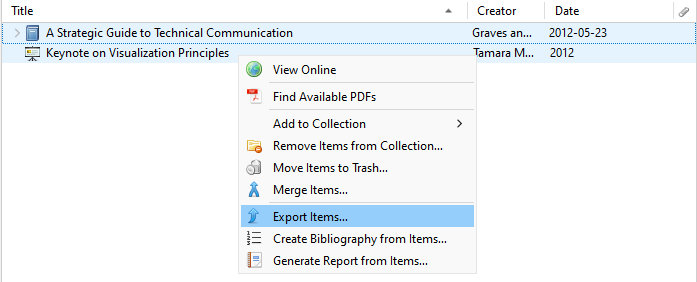
\includegraphics[width=\textwidth]{figures/Figure3-ZoteroBibliographyExport.png}
    \caption{The context menu of chosen sources in Zotero.}
    \label{fig:zoteroContext}
\end{figure}

After this, Zotero exports your chosen sources into a \verb|.bib|. The contents of that file you can copy into the \verb|references.bib| file in this environment. After that, referencing those sources in your text is already working. For each source, Zotero assigns a short label, which you can use to reference it. For example, the command \verb|\cite{tamara_munzner_keynote_2012}| has been used to create a reference to Tamara Munzner's lecture in this template.

The referenced scientific papers usually have Document Object Identifier (DOI) numbers. Specific DOI links\footnote{\url{https://dx.doi.org/}} (in the form doi.org/[number]) are generated from these. When referencing scientific papers, it is recommended to add the DOI links to the reference without the access date. When adding source links, ensure the links are correct and working. When You use the university proxy to access the papers, Your links directly on the browser’s address bar could be proxy links. Do not copy these into Your thesis. Ensure that Your reference links are clean and working, and, when possible, prefer the DOI links.

\subsection{Appendices}
The Appendices section in Your thesis follows the References section. In that part You can present larger tables or screenshots that do not fit in the main contents. Often, it is reasonable to present Your Glossary to define the jargon terms used in Your thesis. If You have created software during Your work, the Appendices section can also include the installation instructions and user manual. The section can be subsectioned and numbered in Your preferred way. For example, Appendix I: Glossary or Appendix B – User Manual, etc. There are many guides to creating a good user manual, but one example of writing technical texts is the textbook „A Strategic Guide to Technical Communication“ by Graves and Graves~\cite{graves_strategic_2012}.

One very important appendix is the description of the accompanying files. Together with the thesis document, You can also add an archived file. That archive file usually includes longer texts (for example, if Your user manual is very long, You need to include longer license texts for the user assets, the questionnaire used in Your study, etc.), larger files (for example, the measured raw data, their analysis files, audio and video recordings of the software or its testing, etc.), the created software, its source code, design concepts and other files created during Your work. Use one of the appendices to describe the contents of the accompanying files.

\subsection{License} \label{subchapter:license}
After the Appendix section, at the end of Your document, You must add a license to allow the  University of Tartu to store and distribute Your thesis. The text of that license is updated often and depends on whether Your work is classified or not. The newest texts are at the URL:  \url{https://adr.ut.ee/?page=pub_list_dynobj&desktop=57835&tid=70993&data_only=true&search=Otsi&field_100193_search_type=ANY&field_100193_text_search_value=ppimine}

The link above has the non-exclusive license as document number 30. In most cases, that license should apply to You. When Your work includes information that must not be published during some timeframe or even indefinitely, You need to write a corresponding application to the vice dean for academic affairs to use a limiting license. The application is in document number 32, and when the vice dean of academic affairs has approved Your application, You can use the corresponding limiting license from document number 31.

\subsection{Metadata}
Your thesis file includes metadata – data about the file itself. This template adds them automatically based on the fields you have written in the \verb|thesis.tex| file. You can see the metadata of a PDF file with the Acrobad Reader software, when you choose \emph{Document Properties} from the context menu of the opened document (see Figure~\ref{fig:metadata}). It is important that the metadata of your work correspond to reality.

\begin{figure}[ht]
    \centering
    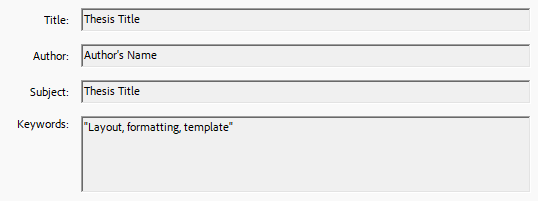
\includegraphics[width=0.8\textwidth]{figures/Figure4-Metadata.png}
    \caption{The metadata of the tempalte in Acrobat Reader.}
    \label{fig:metadata}
\end{figure}

It is recommended that You check through the rest of the metadata to ensure it is all good. For example, it has happened that the author of the file has not been the author of the thesis. This kind of contradiction creates suspicion about who has really authored the thesis document.

%\section{Text Creation} \label{textCreation}
By the time You start using this template, You have likely completed its contents using a more comfortable and collaborative software like Google Docs. Starting formatting makes sense only when the contents of Your work no longer change much. Otherwise, the changes in the content may require doing the formatting part again. Still, some formatting-related recommendations are relevant a lot earlier than when formatting the draft to a fair copy.

\subsection{Chapters}
Your thesis chapters should be evenly balanced with each other. Because this template focuses on formatting, then that guideline is broken here (the previous chapter~\ref{formatting} is noticeably lengthier than this chapter~\ref{textCreation}). In Your work, all the chapters besides the Introduction and Conclusion should have a relatively even length. This principle also helps You not overdo a single part of Your work but spread Your attention to all the essential parts. What precisely these parts are depends on Your thesis type. The University of Tartu’s Institute of Computer Science’s thesis preparation and grading guidelines document defines a certain number of these types. The study or research group where You are doing Your thesis might define continuations of those types. Ensure that Your thesis document provides a balanced coverage of all Your chosen thesis type requires.

\begin{wrapfigure}{r}{0.33\textwidth}
    \centering
    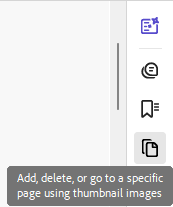
\includegraphics[width=0.33\textwidth]{figures/Figure5-AcrobatReaderMenu.png}
    \caption{The right-hand menu of Acrobat Reader.}
    \label{fig:acrobatReaderMenu}
\end{wrapfigure}
By the time Your thesis starts to take shape, it is useful to look at Your document as a whole. This can be done, for example, with the page order changing tool (\emph{Add, delete, or go to specific page using thumbnail images}) in the Acrobat Reader PDF viewer. The view from that tool shows You Your thesis as a whole. Just like if You would have printed out all of the pages and spread them across a desk. From that view, You see if all the different parts of the document are balanced and in visual equilibrium (see Figure~\ref{fig:acrobatReaderOverview}).

Seda saab teha näiteks Acrobat Reader PDF vaaturis lehekülgede järjekorra muutmise (\emph{Add, delete, or go to specific page using thumbnail images}) tööriistaga (vt joonis~\ref{fig:acrobatReaderMenu}). Tolle tööriista kuva näitab Teile tervet Teie tööd ülevaatlikult. Justkui oleksite oma töö välja printinud ja kõik lehed eraldi suure laua peale laotanud. Sellest ülevaatest Te näete, kas Teie erinevad töö osad on omavahel tasakaalus ja visuaalselt kooskõlas (vt joonis~\ref{fig:acrobatReaderOverview}).

\begin{figure}[t]
    \centering
    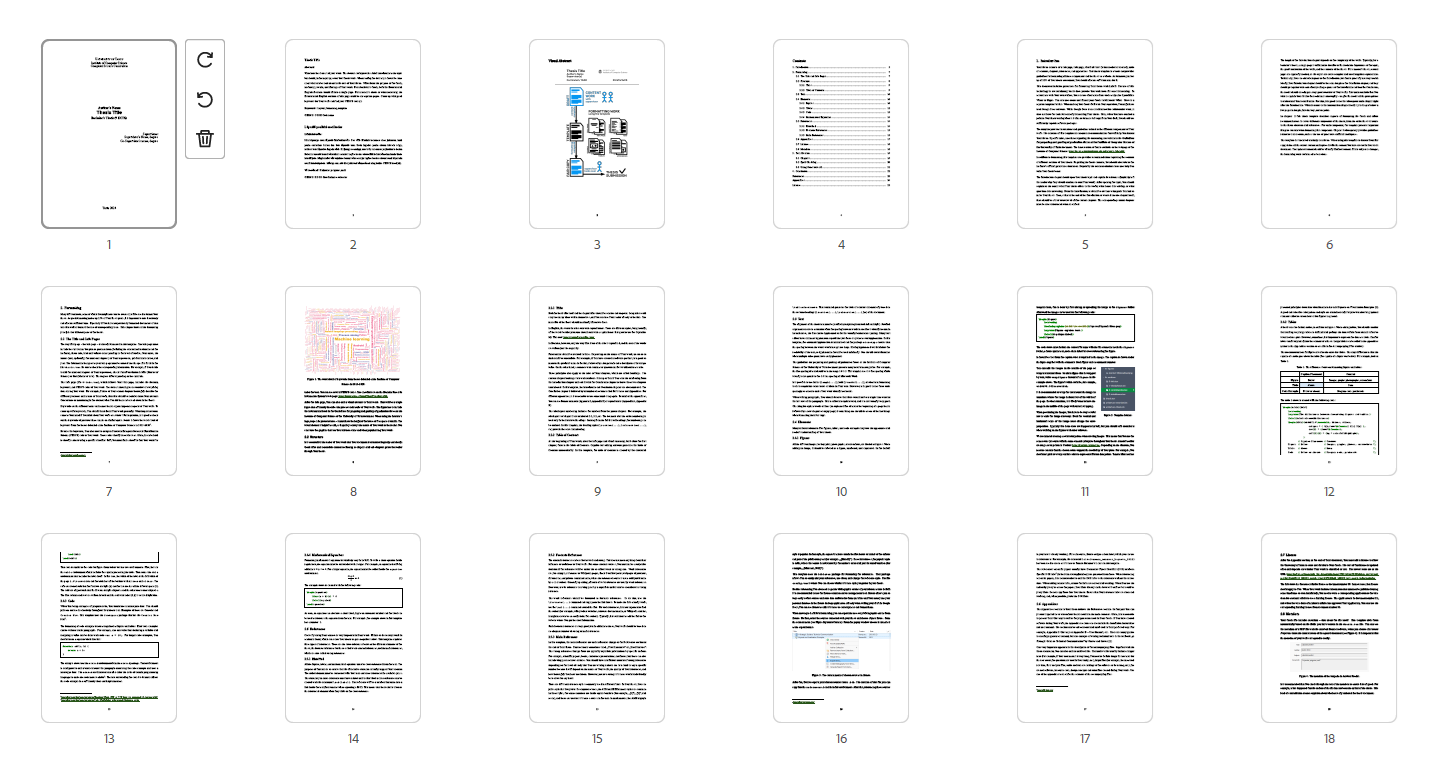
\includegraphics[width=\textwidth]{figures/Figure6-AcrobatReaderOverview.png}
    \caption{The overview of the thesis template in Acrobat Reader.}
    \label{fig:acrobatReaderOverview}
\end{figure}
he birds-eye view of the thesis also shows You if all the necessary places have text. For example, every chapter should start with a brief introductory text. This text must be after the   heading and before any subheadings. That introductory text usually explains why the corresponding chapter is necessary for Your work and what the reader can expect from the subchapters. In addition to that, the (sub)chapters could be woven together with connective sentences, and every bigger chapter could end with a conclusive paragraph. No chapter should start or end with any elements (figures, tables, code examples, equations) or a list. Your thesis text must be smooth to read.

\subsection{Spell Checking}
Microsoft Word’s speller, which You should turn on, comes in really handy when formatting Your fair copy. Having worked on Your draft a lot, You might have gotten used to looking at the same text over and over again; thus, noticing spelling mistakes Yourself might be quite difficult. There are spelling and proofing tools in Word for both the Estonian and English languages. Presenting a thesis that has grammatical errors can result in a lower grade.

Of course, You are also free to use tools that provide grammatical assistance, such as Grammarly, if You have access to such tools, and they make Your work more effective.

\subsection{Using Generative AI}
Using generative AI tools can also make Your work more effective. Here, their use for purely text editing purposes is focused on. When You have also used generative AI for content-related purposes (for example, to create Your questionnaire questions), You should definitely detail Your generative AI usage within the contents of Your thesis text. However, using it for editing Your thesis text is not content-related, so it will suffice to mention its use at the end of the Introduction chapter.

One good way to use a generative AI chatbot is to give it a paragraph of Your text and a prompt to make the specified academic text more readable. When doing that, You should read the result and correct it as needed. The AI chatbot might have mutated Your thoughts in the text, and You must restore them. Also, You might not personally agree with the specific style that AI has provided You and may want to keep tweaking it. The generative AI tools can very effectively help improve Your text flow, but You have to be very keen to ensure that the modified text still conveys Your thoughts and that You agree with the proposed writing style.

It is certainly not effective to use paragraphs that are solely generated by AI in Your thesis text. The author of the thesis is still You. This means that You are responsible for what is written in Your document. Typically, the text written by AI tends to be too general, overly illustrative and includes factual errors that a knowledgeable human author would not make. You do not want to put Yourself into a situation where You have to direct blame towards an AI chatbot due to issues in Your thesis text.

\section{Conclusion} \label{Conclusion}

\section{Discussion}

While an initial solution has been successfully implemented, there remains considerable scope for further development and enhancement.

\subsection{Future Development Opportunities}

Several potential approaches could address the current 12-hour session limitation by exploring alternative authentication flows and API endpoints. One avenue for investigation would involve reverse-engineering the official \textit{eesti.ee} Android application to analyze its authentication mechanisms, for example by decompiling its APK and studying the resulting source code. The application is known to support biometric authentication with PIN code fallback functionality. Through proper reverse engineering and reimplementation of these authentication flows, it may be theoretically possible to automate PIN code resubmission and maintain indefinite session validity.

However, such an approach would constitute a substantial undertaking that could warrant a separate research project. Additionally, this method would likely introduce significantly greater implementation complexity compared to the current solution, potentially making it more fragile and maintenance-intensive.

\subsection{Optimal Solution}

The most effective solution would be for RIA (Information System Authority) to implement equivalent functionality directly within the \textit{eesti.ee} platform. Such an official implementation would be relatively straightforward to develop and would provide superior reliability and future-proofing compared to any third-party solution, including the one presented in this thesis.
\clearpage
\printbibliography[heading=bibintoc]
\section{Glossary}

\subsection{Estonian Government and Technology Terms}

\begin{description}
    \item[\textit{Andmejälgija}] Data Tracker - Protocol developed by RIA for tracking personal data access across state databases.
    
    \item[\textit{\href{https://www.eesti.ee}{eesti.ee}}] Official Estonian state portal providing access to various government e-services.
    
    \item[\textit{TARA}] Trusted Authentication and Authorization service - Estonian government service that handles initial user authentication using strong authentication methods (ID-card, Mobile-ID, Smart-ID, EU eID).
    
    \item[\textit{GovSSO}] Government Single Sign-On service - Manages session state and enables users to access multiple Estonian government e-services with a single authentication. Works in conjunction with TARA to provide seamless access across government platforms.
    
    \item[\textit{Digiregistratuur}] Digital patient registry system in Estonia.
    
    \item[\textit{Rahvastikuregister}] Estonian Population Register.
    
    \item[\textit{E-File} (\textit{E-Toimik})] An information system that provides an overview of the different phases of criminal, civil, administrative and misdemeanour proceedings, procedural acts and court adjudications to all parties involved, including citizens and their representatives \cite{e-file-rik}. Includes the data access tracker for Criminal Records Database.
    
    \item[RIA] \textit{Riigi Infosüsteemi Amet} (Information System Authority) - Estonian government agency responsible for information systems.
    
    \item[X-Road (\textit{X-tee})] Estonian data exchange platform that enables secure data exchange between information systems.
    
    \item[eIDAS] Electronic Identification, Authentication and Trust Services - EU regulation for electronic identification and trust services.
\end{description}

\subsection{Android Development Terms}

\begin{description}
    \item[AlarmManager] Android system service for scheduling operations to be executed at specific times.
    
    \item[WorkManager] Android Jetpack library for deferrable, guaranteed background work. Uses JobScheduler for API 23+, and AlarmManager + BroadcastReceiver for API 14-22. Automatically chooses the best execution method based on Android version and system constraints \cite{android-workmanager}.
    
    \item[Foreground Service] Android service that runs in the background but displays a persistent notification to the user, making the user aware of the ongoing operation. Despite running in the background, it is called ``foreground" because it maintains user visibility through the notification.
    
    \item[Background Service] Android service that runs without user awareness and without displaying notifications. These services are heavily restricted by the system to preserve battery life and system performance.
    
    \item[WebView] Android component that displays web content within an application.
    
    \item[OkHttp] HTTP client library for Android and Java applications.
    
    \item[Proto Data Store] Android library for storing typed objects using Protocol Buffers.
    
    \item[Doze Mode] Android power-saving feature that defers background CPU and network activity for applications.
    
    \item[APK] Android Package - File format used to distribute and install applications on Android.
    
    \item[JWT] JSON Web Token - Method for transmitting information between parties as a signed JSON object.
\end{description}

%\section*{Appendices} \label{appendices} \addcontentsline{toc}{section}{Appendices}
You can make separate sub-sections here for Your glossary, description of accompanying files, user manual, large pictures, and tables.
\section*{License} \label{license} \addcontentsline{toc}{section}{License}



\end{document}



